%&preformat-disser
\RequirePackage[l2tabu,orthodox]{nag} % Раскомментировав, можно в логе получать рекомендации относительно правильного использования пакетов и предупреждения об устаревших и нерекомендуемых пакетах
% Формат А4, 14pt (ГОСТ Р 7.0.11-2011, 5.3.6)
\documentclass[a4paper,14pt,oneside,openany]{memoir}

% все настройки 
% файл с настройками документов, для того чтобы транслировать разные настройки по нескольким документам
% основан на шаблоне диссертации  https://github.com/AndreyAkinshin/Russian-Phd-LaTeX-Dissertation-Template
% Хабибуллин Ринат 2020

% version definition
\newcommand{\unf}{Unifloc 7.17 VBA}



%настройки из Russian-Phd-LaTeX-Dissertation-Template
%%%%%%%%%%%%%%%%%%%%%%%%%%%%%%%%%%%%%%%%%%%%%%%%%%%%%%%%%%%%%%%%%%%%%%%%%%%%%%%%
%%%% Файл упрощённых настроек шаблона, общих для диссертации и автореферата %%%%
%%%%%%%%%%%%%%%%%%%%%%%%%%%%%%%%%%%%%%%%%%%%%%%%%%%%%%%%%%%%%%%%%%%%%%%%%%%%%%%%

%%% Режим черновика %%%
\makeatletter
\@ifundefined{c@draft}{
	\newcounter{draft}
	\setcounter{draft}{0}  % 0 --- чистовик (максимальное соблюдение ГОСТ)
	% 1 --- черновик (отклонения от ГОСТ, но быстрая
	%       сборка итоговых PDF)
}{}
\makeatother

%%% Использование в pdflatex шрифтов не по-умолчанию %%%
\makeatletter
\@ifundefined{c@usealtfont}{
	\newcounter{usealtfont}
	\setcounter{usealtfont}{1}    % 0 --- шрифты на базе Computer Modern
	% 1 --- использовать пакет pscyr, при его
	%       наличии
	% 2 --- использовать пакет XCharter, при наличии
	%       подходящей версии
}{}
\makeatother

%%% Использование в xelatex и lualatex семейств шрифтов %%%
\makeatletter
\@ifundefined{c@fontfamily}{
	\newcounter{fontfamily}
	\setcounter{fontfamily}{1}  % 0 --- CMU семейство. Используется как fallback;
	% 1 --- Шрифты от MS (Times New Roman и компания)
	% 2 --- Семейство Liberation
}{}
\makeatother

%%% Библиография %%%
\makeatletter
\@ifundefined{c@bibliosel}{
	\newcounter{bibliosel}
	\setcounter{bibliosel}{1}   % 0 --- встроенная реализация с загрузкой файла
	%       через движок bibtex8;
	% 1 --- реализация пакетом biblatex через движок
	%       biber
}{}
\makeatother

%%% Предкомпиляция tikz рисунков для ускорения работы %%%
\makeatletter
\@ifundefined{c@imgprecompile}{
	\newcounter{imgprecompile}
	\setcounter{imgprecompile}{0}   % 0 --- без предкомпиляции;
	% 1 --- пользоваться предварительно
	%       скомпилированными pdf вместо генерации
	%       заново из tikz
}{}
\makeatother
            % общие настройки шаблона  
%%% Проверка используемого TeX-движка %%%
\newif\ifxetexorluatex   % определяем новый условный оператор (http://tex.stackexchange.com/a/47579)
\ifxetex
    \xetexorluatextrue
\else
    \ifluatex
        \xetexorluatextrue
    \else
        \xetexorluatexfalse
    \fi
\fi

\newif\ifsynopsis           % Условие, проверяющее, что документ --- автореферат

\usepackage{etoolbox}[2015/08/02]               % Для продвинутой проверки разных условий
\providebool{presentation}

%%% Поля и разметка страницы %%%
\usepackage{pdflscape}                              % Для включения альбомных страниц
\usepackage{geometry}                               % Для последующего задания полей

%%% Математические пакеты %%%
\usepackage{amsthm,amsmath,amscd}   % Математические дополнения от AMS
\usepackage{amsfonts,amssymb}       % Математические дополнения от AMS
\usepackage{mathtools}              % Добавляет окружение multlined
\usepackage{xfrac}                  % Красивые дроби
\usepackage[
    locale = DE,
    list-separator       = {;\,},
    list-final-separator = {;\,},
    list-pair-separator  = {;\,},
    range-phrase={\text{\ensuremath{-}}},
    % quotient-mode        = fraction, % красивые дроби могут не соответствовать ГОСТ
    fraction-function    = \sfrac,
    separate-uncertainty,
    ]{siunitx}                      % Размерности SI
\sisetup{inter-unit-product = \ensuremath{{}\cdot{}}}

% Кириллица в нумерации subequations
% Для правильной работы требуется выполнение сразу после загрузки пакетов
\patchcmd{\subequations}{\def\theequation{\theparentequation\alph{equation}}}
{\def\theequation{\theparentequation\asbuk{equation}}}
{\typeout{subequations patched}}{\typeout{subequations not patched}}

%%%% Установки для размера шрифта 14 pt %%%%
%% Формирование переменных и констант для сравнения (один раз для всех подключаемых файлов)%%
%% должно располагаться до вызова пакета fontspec или polyglossia, потому что они сбивают его работу
\newlength{\curtextsize}
\newlength{\bigtextsize}
\setlength{\bigtextsize}{13.9pt}

\makeatletter
%\show\f@size                                       % неплохо для отслеживания, но вызывает стопорение процесса, если документ компилируется без команды  -interaction=nonstopmode
\setlength{\curtextsize}{\f@size pt}
\makeatother

%%% Кодировки и шрифты %%%
\ifxetexorluatex
    \PassOptionsToPackage{no-math}{fontspec}        % https://tex.stackexchange.com/a/26295/104425
    \usepackage{polyglossia}[2014/05/21]            % Поддержка многоязычности (fontspec подгружается автоматически)
\else
   %%% Решение проблемы копирования текста в буфер кракозябрами
    \ifnumequal{\value{usealtfont}}{0}{}{
        \input glyphtounicode.tex
        \input glyphtounicode-cmr.tex %from pdfx package
        \pdfgentounicode=1
    }
    \usepackage{cmap}                               % Улучшенный поиск русских слов в полученном pdf-файле
    \ifnumequal{\value{usealtfont}}{2}{}{
        \defaulthyphenchar=127                      % Если стоит до fontenc, то переносы не впишутся в выделяемый текст при копировании его в буфер обмена
    }
    \usepackage{textcomp}
    \usepackage[T1,T2A]{fontenc}                    % Поддержка русских букв
    \ifnumequal{\value{usealtfont}}{1}{% Используется pscyr, при наличии
        \IfFileExists{pscyr.sty}{\usepackage{pscyr}}{}  % Подключение pscyr
    }{}
    \usepackage[utf8]{inputenc}[2014/04/30]         % Кодировка utf8
    \usepackage[english, russian]{babel}[2014/03/24]% Языки: русский, английский
    \ifnumequal{\value{usealtfont}}{2}{
        % http://dxdy.ru/post1238763.html#p1238763
        \usepackage[scaled=0.960]{XCharter}[2017/12/19] % Подключение русифицированных шрифтов XCharter
        \usepackage[charter, vvarbb, scaled=1.048]{newtxmath}[2017/12/14]
        \ifpresentation
        \else
            \setDisplayskipStretch{-0.078}
        \fi
    }{}
\fi

%%% Оформление абзацев %%%
\usepackage{indentfirst}                            % Красная строка

%%% Цвета %%%
\ifpresentation
\else
    \usepackage[dvipsnames, table, hyperref]{xcolor} % Совместимо с tikz
\fi

%%% Таблицы %%%
\usepackage{longtable,ltcaption} % Длинные таблицы
\usepackage{multirow,makecell}   % Улучшенное форматирование таблиц
\usepackage{tabu, tabulary}      % таблицы с автоматически подбирающейся
                                 % шириной столбцов (tabu обязательно
                                 % до hyperref вызывать)
\usepackage{threeparttable}      % автоматический подгон ширины подписи таблицы

%%% Общее форматирование
\usepackage{soulutf8}                               % Поддержка переносоустойчивых подчёркиваний и зачёркиваний
\usepackage{icomma}                                 % Запятая в десятичных дробях

%%% Оптимизация расстановки переносов и длины последней строки абзаца
\IfFileExists{impnattypo.sty}{% проверка установленности пакета impnattypo
    \ifluatex
        \ifnumequal{\value{draft}}{1}{% Черновик
            \usepackage[hyphenation, lastparline, nosingleletter, homeoarchy,
            rivers, draft]{impnattypo}
        }{% Чистовик
            \usepackage[hyphenation, lastparline, nosingleletter]{impnattypo}
        }
    \else
        \usepackage[hyphenation, lastparline]{impnattypo}
    \fi
}{}

%% Векторная графика

\usepackage{tikz}                   % Продвинутый пакет векторной графики
\usetikzlibrary{chains}             % Для примера tikz рисунка
\usetikzlibrary{shapes.geometric}   % Для примера tikz рисунка
\usetikzlibrary{shapes.symbols}     % Для примера tikz рисунка
\usetikzlibrary{arrows}             % Для примера tikz рисунка

%%% Гиперссылки %%%
\usepackage{hyperref}[2012/11/06]

%%% Изображения %%%
\usepackage{graphicx}[2014/04/25]                   % Подключаем пакет работы с графикой

%%% Счётчики %%%
\usepackage[figure,table]{totalcount}               % Счётчик рисунков и таблиц
\usepackage{totcount}                               % Пакет создания счётчиков на основе последнего номера подсчитываемого элемента (может требовать дважды компилировать документ)
\usepackage{totpages}                               % Счётчик страниц, совместимый с hyperref (ссылается на номер последней страницы). Желательно ставить последним пакетом в преамбуле

%%% Продвинутое управление групповыми ссылками (пока только формулами) %%%
\ifpresentation
\else
    \usepackage[russian]{cleveref} % cleveref имеет сложности со считыванием
    % языка из babel. Такое решение русификации вывода выбрано вместо
    % определения в documentclass из опасности что-то лишнее передать во все
    % остальные пакеты, включая библиографию.
    \creflabelformat{equation}{#2#1#3} % Формат по умолчанию ставил круглые
    % скобки вокруг каждого номера ссылки, теперь просто номера ссылок без
    % какого-либо дополнительного оформления
    \crefrangelabelformat{equation}{#3#1#4\cyrdash#5#2#6} % Интервалы в русском
    % языке принято делать через тире, если иное не оговорено

    % решение проблемы с "и" в \labelcref
    % https://tex.stackexchange.com/a/455124/104425
    \ifxetexorluatex
        \DeclareTextSymbol{\cyri}\UnicodeEncodingName{"0438} % и
    \fi

    % Добавление возможности использования пробелов в \labelcref
    % https://tex.stackexchange.com/a/340502/104425
    \usepackage{kvsetkeys}
    \makeatletter
    \let\org@@cref\@cref
    \renewcommand*{\@cref}[2]{%
        \edef\process@me{%
            \noexpand\org@@cref{#1}{\zap@space#2 \@empty}%
        }\process@me
    }
    \makeatother

    \newcommand{\eqrefs}[1]{(\labelcref{#1})}
    \newcommand{\refs}[1]{\labelcref{#1}}
\fi

\ifnumequal{\value{draft}}{1}{% Черновик
    \usepackage[firstpage]{draftwatermark}
    \SetWatermarkText{DRAFT}
    \SetWatermarkFontSize{14pt}
    \SetWatermarkScale{15}
    \SetWatermarkAngle{45}
}{}

%%% Исправление положения якорей подписей (под)рисунков %%%
% Без hypcap и патча, при клике по ссылке на подрисунок, просмотрщик pdf прыгает "к подписи" а не "к рисунку".
% Подробнее: https://github.com/AndreyAkinshin/Russian-Phd-LaTeX-Dissertation-Template/issues/238
% (!) Даже с патчем, если мешать в одной фиге разные типы подфиг (subbottom и subcaption) - ссылки всё равно будут работать неправильно  (см. https://www.overleaf.com/read/czmbmmtnqrrg ).
\ifpresentation
\else
    \usepackage[all]{hypcap}

    \makeatletter
    \ltx@ifclasslater{memoir}{2018/12/13}{
        % Предполагается, что в следующей версии класс будет исправлен
        \typeout{Assuming this version of memoir is free from the jumping-to-caption bug.}
    }{
        \usepackage{xpatch}

        \newcommand\mem@step@subcounter{\refstepcounter{sub\@captype}\@contkeep}

        \xpatchcmd{\@memsubbody}%
        {\refstepcounter{sub\@captype}\@contkeep}% search pattern
        {}% replacement
        {\typeout{@memsubbody is patched}}%
        {\typeout{@memsubbody is NOT patched}}%

        \xpatchcmd{\@memcontsubbody}%
        {\refstepcounter{sub\@captype}\@contkeep}% pattern
        {}% replacement
        {\typeout{@memcontsubbody is patched}}%
        {\typeout{@memcontsubbody is NOT patched}}%

        \xpatchcmd{\@memsubfloat}%
        {\vbox\bgroup}% search pattern
        {\vbox\bgroup\mem@step@subcounter}% replacement
        {\typeout{@memsubfloat patch is ok}}%
        {\typeout{@memsubfloat patch is NOT ok}}%

        \xpatchcmd{\subcaption}%
        {\refstepcounter{sub\@captype}}% search pattern
        {\H@refstepcounter{sub\@captype}}% replacement
        {\typeout{subcaption second patch is ok}}%
        {\typeout{subcaption second patch is NOT ok}}%
    }
    \makeatother
\fi

%%% Цитата, не приводимая в автореферате:
% возможно, актуальна только для biblatex
%\newcommand{\citeinsynopsis}[1]{\ifsynopsis\else ~\cite{#1} \fi}

% если текущий процесс запущен библиотекой tikz-external, то прекомпиляция должна быть включена
\ifdefined\tikzexternalrealjob
    \setcounter{imgprecompile}{1}
\fi

\ifnumequal{\value{imgprecompile}}{1}{% Только если у нас включена предкомпиляция
    \usetikzlibrary{external}   % подключение возможности предкомпиляции
    \tikzexternalize[prefix=images/cache/] % activate! % здесь можно указать отдельную папку для скомпилированных файлов
    \ifxetex
        \tikzset{external/up to date check={diff}}
    \fi
}{}
         % Пакеты общие для диссертации и автореферата 
%%% Прикладные пакеты %%%
%\usepackage{calc}               % Пакет для расчётов параметров, например длины

%%% Для добавления Стр. над номерами страниц в оглавлении
%%% http://tex.stackexchange.com/a/306950
\usepackage{afterpage}

%%% Списки %%%
\usepackage{enumitem}
      % Пакеты общие для диссертации и автореферата
\usepackage{fr-longtable}    %ради \endlasthead

% Листинги с исходным кодом программ
\usepackage{fancyvrb}
\usepackage{listings}
\lccode`\~=0\relax %Без этого хака из-за особенностей пакета listings перестают работать конструкции с \MakeLowercase и т. п. в (xe|lua)latex

% Русская традиция начертания греческих букв
\usepackage{upgreek} % прямые греческие ради русской традиции

%%% Микротипографика
%\ifnumequal{\value{draft}}{0}{% Только если у нас режим чистовика
%    \usepackage[final, babel, shrink=45]{microtype}[2016/05/14] % улучшает представление букв и слов в строках, может помочь при наличии отдельно висящих слов
%}{}

% Отметка о версии черновика на каждой странице
% Чтобы работало надо в своей локальной копии по инструкции
% https://www.ctan.org/pkg/gitinfo2 создать небходимые файлы в папке
% ./git/hooks
% If you’re familiar with tweaking git, you can probably work it out for
% yourself. If not, I suggest you follow these steps:
% 1. First, you need a git repository and working tree. For this example,
% let’s suppose that the root of the working tree is in ~/compsci
% 2. Copy the file post-xxx-sample.txt (which is in the same folder of
% your TEX distribution as this pdf) into the git hooks directory in your
% working copy. In our example case, you should end up with a file called
% ~/compsci/.git/hooks/post-checkout
% 3. If you’re using a unix-like system, don’t forget to make the file executable.
% Just how you do this is outside the scope of this manual, but one
% possible way is with commands such as this:
% chmod g+x post-checkout.
% 4. Test your setup with “git checkout master” (or another suitable branch
% name). This should generate copies of gitHeadInfo.gin in the directories
% you intended.
% 5. Now make two more copies of this file in the same directory (hooks),
% calling them post-commit and post-merge, and you’re done. As before,
% users of unix-like systems should ensure these files are marked as
% executable.
\ifnumequal{\value{draft}}{1}{% Черновик
   \IfFileExists{.git/gitHeadInfo.gin}{
      \usepackage[mark,pcount]{gitinfo2}
      \renewcommand{\gitMark}{rev.\gitAbbrevHash\quad\gitCommitterEmail\quad\gitAuthorIsoDate}
      \renewcommand{\gitMarkFormat}{\rmfamily\color{Gray}\small\bfseries}
   }{}
}{}     % Пакеты общие для диссертации и автореферата
%%%%%%%%%%%%%%%%%%%%%%%%%%%%%%%%%%%%%%%%%%%%%%%%%%%%%%
%%%% Файл упрощённых настроек шаблона диссертации %%%%
%%%%%%%%%%%%%%%%%%%%%%%%%%%%%%%%%%%%%%%%%%%%%%%%%%%%%%

%%% Инициализирование переменных, не трогать!  %%%
\newcounter{intvl}
\newcounter{otstup}
\newcounter{contnumeq}
\newcounter{contnumfig}
\newcounter{contnumtab}
\newcounter{pgnum}
\newcounter{chapstyle}
\newcounter{headingdelim}
\newcounter{headingalign}
\newcounter{headingsize}
\newcounter{tabcap}
\newcounter{tablaba}
\newcounter{tabtita}
%%%%%%%%%%%%%%%%%%%%%%%%%%%%%%%%%%%%%%%%%%%%%%%%%%%%%%

%%% Область упрощённого управления оформлением %%%

%% Интервал между заголовками и между заголовком и текстом %%
% Заголовки отделяют от текста сверху и снизу
% тремя интервалами (ГОСТ Р 7.0.11-2011, 5.3.5)
\setcounter{intvl}{3}               % Коэффициент кратности к размеру шрифта

%% Отступы у заголовков в тексте %%
\setcounter{otstup}{0}              % 0 --- без отступа; 1 --- абзацный отступ

%% Нумерация формул, таблиц и рисунков %%
% Нумерация формул
\setcounter{contnumeq}{0}   % 0 --- пораздельно (во введении подряд,
                            %       без номера раздела);
                            % 1 --- сквозная нумерация по всей диссертации
% Нумерация рисунков
\setcounter{contnumfig}{0}  % 0 --- пораздельно (во введении подряд,
                            %       без номера раздела);
                            % 1 --- сквозная нумерация по всей диссертации
% Нумерация таблиц
\setcounter{contnumtab}{1}  % 0 --- пораздельно (во введении подряд,
                            %       без номера раздела);
                            % 1 --- сквозная нумерация по всей диссертации

%% Оглавление %%
\setcounter{pgnum}{1}       % 0 --- номера страниц никак не обозначены;
                            % 1 --- Стр. над номерами страниц (дважды
                            %       компилировать после изменения настройки)
\settocdepth{subsection}    % до какого уровня подразделов выносить в оглавление
\setsecnumdepth{subsection} % до какого уровня нумеровать подразделы


%% Текст и форматирование заголовков %%
\setcounter{chapstyle}{1}     % 0 --- разделы только под номером;
                              % 1 --- разделы с названием "Глава" перед номером
\setcounter{headingdelim}{1}  % 0 --- номер отделен пропуском в 1em или \quad;
                              % 1 --- номера разделов и приложений отделены
                              %       точкой с пробелом, подразделы пропуском
                              %       без точки;
                              % 2 --- номера разделов, подразделов и приложений
                              %       отделены точкой с пробелом.

%% Выравнивание заголовков в тексте %%
\setcounter{headingalign}{0}  % 0 --- по центру;
                              % 1 --- по левому краю

%% Размеры заголовков в тексте %%
\setcounter{headingsize}{0}   % 0 --- по ГОСТ, все всегда 14 пт;
                              % 1 --- пропорционально изменяющийся размер
                              %       в зависимости от базового шрифта

%% Подпись таблиц %%
\setcounter{tabcap}{0}  % 0 --- по ГОСТ, номер таблицы и название разделены
                        %       тире, выровнены по левому краю, при
                        %       необходимостина нескольких строках;
                        % 1 --- подпись таблицы не по ГОСТ, на двух и более
                        %       строках, дальнейшие настройки:
%Выравнивание первой строки, с подписью и номером
\setcounter{tablaba}{2} % 0 --- по левому краю;
                        % 1 --- по центру;
                        % 2 --- по правому краю
%Выравнивание строк с самим названием таблицы
\setcounter{tabtita}{1} % 0 --- по левому краю;
                        % 1 --- по центру;
                        % 2 --- по правому краю
%Разделитель записи «Таблица #» и названия таблицы
\newcommand{\tablabelsep}{ }

%% Подпись рисунков %%
%Разделитель записи «Рисунок #» и названия рисунка
\newcommand{\figlabelsep}{~\cyrdash\ }  % (ГОСТ 2.105, 4.3.1)
                                        % "--- здесь не работает

%%% Цвета гиперссылок %%%
% Latex color definitions: http://latexcolor.com/
\definecolor{linkcolor}{rgb}{0.9,0,0}
\definecolor{citecolor}{rgb}{0,0.6,0}
\definecolor{urlcolor}{rgb}{0,0,1}
%\definecolor{linkcolor}{rgb}{0,0,0} %black
%\definecolor{citecolor}{rgb}{0,0,0} %black
%\definecolor{urlcolor}{rgb}{0,0,0} %black
   % Упрощённые настройки шаблона  
% Новые переменные, которые могут использоваться во всём проекте
% ГОСТ 7.0.11-2011
% 9.2 Оформление текста автореферата диссертации
% 9.2.1 Общая характеристика работы включает в себя следующие основные структурные
% элементы:
% актуальность темы исследования;
\newcommand{\actualityTXT}{Актуальность темы.}
% степень ее разработанности;
\newcommand{\progressTXT}{Степень разработанности темы.}
% цели и задачи;
\newcommand{\aimTXT}{Целью}
\newcommand{\tasksTXT}{задачи}
% научную новизну;
\newcommand{\noveltyTXT}{Научная новизна:}
% теоретическую и практическую значимость работы;
%\newcommand{\influenceTXT}{Теоретическая и практическая значимость}
% или чаще используют просто
\newcommand{\influenceTXT}{Практическая значимость}
% методологию и методы исследования;
\newcommand{\methodsTXT}{Методология и методы исследования.}
% положения, выносимые на защиту;
\newcommand{\defpositionsTXT}{Основные положения, выносимые на~защиту:}
% степень достоверности и апробацию результатов.
\newcommand{\reliabilityTXT}{Достоверность}
\newcommand{\probationTXT}{Апробация работы.}

\newcommand{\contributionTXT}{Личный вклад.}
\newcommand{\publicationsTXT}{Публикации.}


%%% Заголовки библиографии:

% для автореферата:
\newcommand{\bibtitleauthor}{Публикации автора по теме диссертации}

% для стиля библиографии `\insertbiblioauthorgrouped`
\newcommand{\bibtitleauthorvak}{В изданиях из списка ВАК РФ}
\newcommand{\bibtitleauthorscopus}{В изданиях, входящих в международную базу цитирования Scopus}
\newcommand{\bibtitleauthorwos}{В изданиях, входящих в международную базу цитирования Web of Science}
\newcommand{\bibtitleauthorother}{В прочих изданиях}
\newcommand{\bibtitleauthorconf}{В сборниках трудов конференций}

% для стиля библиографии `\insertbiblioauthorimportant`:
\newcommand{\bibtitleauthorimportant}{Наиболее значимые \protect\MakeLowercase\bibtitleauthor}

% для списка литературы в диссертации и списка чужих работ в автореферате:
\newcommand{\bibtitlefull}{Список литературы} % (ГОСТ Р 7.0.11-2011, 4)
         % Новые переменные, для всего проекта
%%% Кодировки и шрифты %%%
\ifxetexorluatex
    \setmainlanguage[babelshorthands=true]{russian}    % Язык по-умолчанию русский с поддержкой приятных команд пакета babel
    \setotherlanguage{english}                         % Дополнительный язык = английский (в американской вариации по-умолчанию)

    % Проверка существования шрифтов. Недоступна в pdflatex
    \ifnumequal{\value{fontfamily}}{1}{
        \IfFontExistsTF{Times New Roman}{}{\setcounter{fontfamily}{0}}
    }{}
    \ifnumequal{\value{fontfamily}}{2}{
        \IfFontExistsTF{LiberationSerif}{}{\setcounter{fontfamily}{0}}
    }{}

    \ifnumequal{\value{fontfamily}}{0}{                    % Семейство шрифтов CMU. Используется как fallback
        \setmonofont{CMU Typewriter Text}                  % моноширинный шрифт
        \newfontfamily\cyrillicfonttt{CMU Typewriter Text} % моноширинный шрифт для кириллицы
        \defaultfontfeatures{Ligatures=TeX}                % стандартные лигатуры TeX, замены нескольких дефисов на тире и т. п. Настройки моноширинного шрифта должны идти до этой строки, чтобы при врезках кода программ в коде не применялись лигатуры и замены дефисов
        \setmainfont{CMU Serif}                            % Шрифт с засечками
        \newfontfamily\cyrillicfont{CMU Serif}             % Шрифт с засечками для кириллицы
        \setsansfont{CMU Sans Serif}                       % Шрифт без засечек
        \newfontfamily\cyrillicfontsf{CMU Sans Serif}      % Шрифт без засечек для кириллицы
    }

    \ifnumequal{\value{fontfamily}}{1}{                    % Семейство MS шрифтов
        \setmonofont{Courier New}                          % моноширинный шрифт
        \newfontfamily\cyrillicfonttt{Courier New}         % моноширинный шрифт для кириллицы
        \defaultfontfeatures{Ligatures=TeX}                % стандартные лигатуры TeX, замены нескольких дефисов на тире и т. п. Настройки моноширинного шрифта должны идти до этой строки, чтобы при врезках кода программ в коде не применялись лигатуры и замены дефисов
        \setmainfont{Times New Roman}                      % Шрифт с засечками
        \newfontfamily\cyrillicfont{Times New Roman}       % Шрифт с засечками для кириллицы
        \setsansfont{Arial}                                % Шрифт без засечек
        \newfontfamily\cyrillicfontsf{Arial}               % Шрифт без засечек для кириллицы
    }

    \ifnumequal{\value{fontfamily}}{2}{                    % Семейство шрифтов Liberation (https://pagure.io/liberation-fonts)
        \setmonofont{LiberationMono}[Scale=0.87] % моноширинный шрифт
        \newfontfamily\cyrillicfonttt{LiberationMono}[     % моноширинный шрифт для кириллицы
            Scale=0.87]
        \defaultfontfeatures{Ligatures=TeX}                % стандартные лигатуры TeX, замены нескольких дефисов на тире и т. п. Настройки моноширинного шрифта должны идти до этой строки, чтобы при врезках кода программ в коде не применялись лигатуры и замены дефисов
        \setmainfont{LiberationSerif}                      % Шрифт с засечками
        \newfontfamily\cyrillicfont{LiberationSerif}       % Шрифт с засечками для кириллицы
        \setsansfont{LiberationSans}                       % Шрифт без засечек
        \newfontfamily\cyrillicfontsf{LiberationSans}      % Шрифт без засечек для кириллицы
    }

\else
    \ifnumequal{\value{usealtfont}}{1}{% Используется pscyr, при наличии
        \IfFileExists{pscyr.sty}{\renewcommand{\rmdefault}{ftm}}{}
    }{}
\fi
            % Определение шрифтов (частичное)
%%% Шаблон %%%
\DeclareRobustCommand{\todo}{\textcolor{red}}       % решаем проблему превращения названия цвета в результате \MakeUppercase, http://tex.stackexchange.com/a/187930, \DeclareRobustCommand protects \todo from expanding inside \MakeUppercase
\AtBeginDocument{%
    \setlength{\parindent}{2.5em}                   % Абзацный отступ. Должен быть одинаковым по всему тексту и равен пяти знакам (ГОСТ Р 7.0.11-2011, 5.3.7).
}

%%% Подписи %%%
\setlength{\abovecaptionskip}{0pt}   % Отбивка над подписью
\setlength{\belowcaptionskip}{0pt}   % Отбивка под подписью
\captionwidth{\linewidth}
\normalcaptionwidth

%%% Таблицы %%%
\ifnumequal{\value{tabcap}}{0}{%
    \newcommand{\tabcapalign}{\raggedright}  % по левому краю страницы или аналога parbox
    \renewcommand{\tablabelsep}{~\cyrdash\ } % тире как разделитель идентификатора с номером от наименования
    \newcommand{\tabtitalign}{}
}{%
    \ifnumequal{\value{tablaba}}{0}{%
        \newcommand{\tabcapalign}{\raggedright}  % по левому краю страницы или аналога parbox
    }{}

    \ifnumequal{\value{tablaba}}{1}{%
        \newcommand{\tabcapalign}{\centering}    % по центру страницы или аналога parbox
    }{}

    \ifnumequal{\value{tablaba}}{2}{%
        \newcommand{\tabcapalign}{\raggedleft}   % по правому краю страницы или аналога parbox
    }{}

    \ifnumequal{\value{tabtita}}{0}{%
        \newcommand{\tabtitalign}{\par\raggedright}  % по левому краю страницы или аналога parbox
    }{}

    \ifnumequal{\value{tabtita}}{1}{%
        \newcommand{\tabtitalign}{\par\centering}    % по центру страницы или аналога parbox
    }{}

    \ifnumequal{\value{tabtita}}{2}{%
        \newcommand{\tabtitalign}{\par\raggedleft}   % по правому краю страницы или аналога parbox
    }{}
}

\precaption{\tabcapalign} % всегда идет перед подписью или \legend
\captionnamefont{\normalfont\normalsize} % Шрифт надписи «Таблица #»; также определяет шрифт у \legend
\captiondelim{\tablabelsep} % разделитель идентификатора с номером от наименования
\captionstyle[\tabtitalign]{\tabtitalign}
\captiontitlefont{\normalfont\normalsize} % Шрифт с текстом подписи

%%% Рисунки %%%
\setfloatadjustment{figure}{%
    \setlength{\abovecaptionskip}{0pt}   % Отбивка над подписью
    \setlength{\belowcaptionskip}{0pt}   % Отбивка под подписью
    \precaption{} % всегда идет перед подписью или \legend
    \captionnamefont{\normalfont\normalsize} % Шрифт надписи «Рисунок #»; также определяет шрифт у \legend
    \captiondelim{\figlabelsep} % разделитель идентификатора с номером от наименования
    \captionstyle[\centering]{\centering} % Центрирование подписей, заданных командой \caption и \legend
    \captiontitlefont{\normalfont\normalsize} % Шрифт с текстом подписи
    \postcaption{} % всегда идет после подписи или \legend, и с новой строки
}

%%% Подписи подрисунков %%%
\newsubfloat{figure} % Включает возможность использовать подрисунки у окружений figure
\renewcommand{\thesubfigure}{\asbuk{subfigure}}           % Буквенные номера подрисунков
\subcaptionsize{\normalsize} % Шрифт подписи названий подрисунков (не отличается от основного)
\subcaptionlabelfont{\normalfont}
\subcaptionfont{\!\!) \normalfont} % Вот так тут добавили скобку после буквы.
\subcaptionstyle{\centering}
%\subcaptionsize{\fontsize{12pt}{13pt}\selectfont} % объявляем шрифт 12pt для использования в подписях, тут же надо интерлиньяж объявлять, если не наследуется

%%% Настройки гиперссылок %%%
\ifluatex
    \hypersetup{
        unicode,                % Unicode encoded PDF strings
    }
\fi

\hypersetup{
    linktocpage=true,           % ссылки с номера страницы в оглавлении, списке таблиц и списке рисунков
%    linktoc=all,                % both the section and page part are links
%    pdfpagelabels=false,        % set PDF page labels (true|false)
    plainpages=false,           % Forces page anchors to be named by the Arabic form  of the page number, rather than the formatted form
    colorlinks,                 % ссылки отображаются раскрашенным текстом, а не раскрашенным прямоугольником, вокруг текста
    linkcolor={linkcolor},      % цвет ссылок типа ref, eqref и подобных
    citecolor={citecolor},      % цвет ссылок-цитат
    urlcolor={urlcolor},        % цвет гиперссылок
%    hidelinks,                  % Hide links (removing color and border)
%    pdftitle={\thesisTitle},    % Заголовок
%    pdfauthor={\thesisAuthor},  % Автор
%    pdfsubject={\thesisSpecialtyNumber\ \thesisSpecialtyTitle},      % Тема
%    pdfcreator={Создатель},     % Создатель, Приложение
%    pdfproducer={Производитель},% Производитель, Производитель PDF
%    pdfkeywords={\keywords},    % Ключевые слова
    pdflang={ru},
}
\ifnumequal{\value{draft}}{1}{% Черновик
    \hypersetup{
        draft,
    }
}{}

%%% Списки %%%
% Используем короткое тире (endash) для ненумерованных списков (ГОСТ 2.105-95, пункт 4.1.7, требует дефиса, но так лучше смотрится)
\renewcommand{\labelitemi}{\normalfont\bfseries{--}}

% Перечисление строчными буквами латинского алфавита (ГОСТ 2.105-95, 4.1.7)
%\renewcommand{\theenumi}{\alph{enumi}}
%\renewcommand{\labelenumi}{\theenumi)}

% Перечисление строчными буквами русского алфавита (ГОСТ 2.105-95, 4.1.7)
\makeatletter
\AddEnumerateCounter{\asbuk}{\russian@alph}{щ}      % Управляем списками/перечислениями через пакет enumitem, а он 'не знает' про asbuk, потому 'учим' его
\makeatother
%\renewcommand{\theenumi}{\asbuk{enumi}} %первый уровень нумерации
%\renewcommand{\labelenumi}{\theenumi)} %первый уровень нумерации
\renewcommand{\theenumii}{\asbuk{enumii}} %второй уровень нумерации
\renewcommand{\labelenumii}{\theenumii)} %второй уровень нумерации
\renewcommand{\theenumiii}{\arabic{enumiii}} %третий уровень нумерации
\renewcommand{\labelenumiii}{\theenumiii)} %третий уровень нумерации

\setlist{nosep,%                                    % Единый стиль для всех списков (пакет enumitem), без дополнительных интервалов.
    labelindent=\parindent,leftmargin=*%            % Каждый пункт, подпункт и перечисление записывают с абзацного отступа (ГОСТ 2.105-95, 4.1.8)
}

%%% Правильная нумерация приложений, рисунков и формул %%%
%% По ГОСТ 2.105, п. 4.3.8 Приложения обозначают заглавными буквами русского алфавита,
%% начиная с А, за исключением букв Ё, З, Й, О, Ч, Ь, Ы, Ъ.
%% Здесь также переделаны все нумерации русскими буквами.
\ifxetexorluatex
    \makeatletter
    \def\russian@Alph#1{\ifcase#1\or
       А\or Б\or В\or Г\or Д\or Е\or Ж\or
       И\or К\or Л\or М\or Н\or
       П\or Р\or С\or Т\or У\or Ф\or Х\or
       Ц\or Ш\or Щ\or Э\or Ю\or Я\else\xpg@ill@value{#1}{russian@Alph}\fi}
    \def\russian@alph#1{\ifcase#1\or
       а\or б\or в\or г\or д\or е\or ж\or
       и\or к\or л\or м\or н\or
       п\or р\or с\or т\or у\or ф\or х\or
       ц\or ш\or щ\or э\or ю\or я\else\xpg@ill@value{#1}{russian@alph}\fi}
    \def\cyr@Alph#1{\ifcase#1\or
        А\or Б\or В\or Г\or Д\or Е\or Ж\or
        И\or К\or Л\or М\or Н\or
        П\or Р\or С\or Т\or У\or Ф\or Х\or
        Ц\or Ш\or Щ\or Э\or Ю\or Я\else\xpg@ill@value{#1}{cyr@Alph}\fi}
    \def\cyr@alph#1{\ifcase#1\or
        а\or б\or в\or г\or д\or е\or ж\or
        и\or к\or л\or м\or н\or
        п\or р\or с\or т\or у\or ф\or х\or
        ц\or ш\or щ\or э\or ю\or я\else\xpg@ill@value{#1}{cyr@alph}\fi}
    \makeatother
\else
    \makeatletter
    \if@uni@ode
      \def\russian@Alph#1{\ifcase#1\or
        А\or Б\or В\or Г\or Д\or Е\or Ж\or
        И\or К\or Л\or М\or Н\or
        П\or Р\or С\or Т\or У\or Ф\or Х\or
        Ц\or Ш\or Щ\or Э\or Ю\or Я\else\@ctrerr\fi}
    \else
      \def\russian@Alph#1{\ifcase#1\or
        \CYRA\or\CYRB\or\CYRV\or\CYRG\or\CYRD\or\CYRE\or\CYRZH\or
        \CYRI\or\CYRK\or\CYRL\or\CYRM\or\CYRN\or
        \CYRP\or\CYRR\or\CYRS\or\CYRT\or\CYRU\or\CYRF\or\CYRH\or
        \CYRC\or\CYRSH\or\CYRSHCH\or\CYREREV\or\CYRYU\or
        \CYRYA\else\@ctrerr\fi}
    \fi
    \if@uni@ode
      \def\russian@alph#1{\ifcase#1\or
        а\or б\or в\or г\or д\or е\or ж\or
        и\or к\or л\or м\or н\or
        п\or р\or с\or т\or у\or ф\or х\or
        ц\or ш\or щ\or э\or ю\or я\else\@ctrerr\fi}
    \else
      \def\russian@alph#1{\ifcase#1\or
        \cyra\or\cyrb\or\cyrv\or\cyrg\or\cyrd\or\cyre\or\cyrzh\or
        \cyri\or\cyrk\or\cyrl\or\cyrm\or\cyrn\or
        \cyrp\or\cyrr\or\cyrs\or\cyrt\or\cyru\or\cyrf\or\cyrh\or
        \cyrc\or\cyrsh\or\cyrshch\or\cyrerev\or\cyryu\or
        \cyrya\else\@ctrerr\fi}
    \fi
    \makeatother
\fi
           % Стили общие для диссертации и автореферата

%%% Изображения %%%
\graphicspath{{pics/}}

%%% Переопределение именований, если иначе не сработает %%%
%\gappto\captionsrussian{
%    \renewcommand{\chaptername}{Глава}
%    \renewcommand{\appendixname}{Приложение} % (ГОСТ Р 7.0.11-2011, 5.7)
%}



%%% Интервалы %%%
%% По ГОСТ Р 7.0.11-2011, пункту 5.3.6 требуется полуторный интервал
%% Реализация средствами класса (на основе setspace) ближе к типографской классике.
%% И правит сразу и в таблицах (если со звёздочкой)
%\DoubleSpacing*     % Двойной интервал
\OnehalfSpacing*    % Полуторный интервал
%\setSpacing{1.42}   % Полуторный интервал, подобный Ворду (возможно, стоит включать вместе с предыдущей строкой)

%%% Макет страницы %%%
% Выставляем значения полей (ГОСТ 7.0.11-2011, 5.3.7)
\geometry{a4paper, top=2cm, bottom=2cm, left=2.5cm, right=1cm, nofoot, nomarginpar} %, heightrounded, showframe
\setlength{\topskip}{0pt}   %размер дополнительного верхнего поля
\setlength{\footskip}{12.3pt} % снимет warning, согласно https://tex.stackexchange.com/a/334346

%%% Выравнивание и переносы %%%
%% http://tex.stackexchange.com/questions/241343/what-is-the-meaning-of-fussy-sloppy-emergencystretch-tolerance-hbadness
%% http://www.latex-community.org/forum/viewtopic.php?p=70342#p70342
\tolerance 1414
\hbadness 1414
\emergencystretch 1.5em % В случае проблем регулировать в первую очередь
\hfuzz 0.3pt
\vfuzz \hfuzz
%\raggedbottom
%\sloppy                 % Избавляемся от переполнений
\clubpenalty=10000      % Запрещаем разрыв страницы после первой строки абзаца
\widowpenalty=10000     % Запрещаем разрыв страницы после последней строки абзаца
\brokenpenalty=4991     % Ограничение на разрыв страницы, если строка заканчивается переносом

%%% Блок управления параметрами для выравнивания заголовков в тексте %%%
\newlength{\otstuplen}
\setlength{\otstuplen}{\theotstup\parindent}
\ifnumequal{\value{headingalign}}{0}{% выравнивание заголовков в тексте
    \newcommand{\hdngalign}{\centering}                % по центру
    \newcommand{\hdngaligni}{}% по центру
    \setlength{\otstuplen}{0pt}
}{%
    \newcommand{\hdngalign}{}                 % по левому краю
    \newcommand{\hdngaligni}{\hspace{\otstuplen}}      % по левому краю
} % В обоих случаях вроде бы без переноса, как и надо (ГОСТ Р 7.0.11-2011, 5.3.5)

%%% Оглавление %%%
\renewcommand{\cftchapterdotsep}{\cftdotsep}                % отбивка точками до номера страницы начала главы/раздела

%% Переносить слова в заголовке не допускается (ГОСТ Р 7.0.11-2011, 5.3.5). Заголовки в оглавлении должны точно повторять заголовки в тексте (ГОСТ Р 7.0.11-2011, 5.2.3). Прямого указания на запрет переносов в оглавлении нет, но по той же логике невнесения искажений в смысл, лучше в оглавлении не переносить:
\setrmarg{3.55em plus1fil}                             %To have the (sectional) titles in the ToC, etc., typeset ragged right with no hyphenation
\renewcommand{\cftchapterpagefont}{\normalfont}        % нежирные номера страниц у глав в оглавлении
\renewcommand{\cftchapterleader}{\cftdotfill{\cftchapterdotsep}}% нежирные точки до номеров страниц у глав в оглавлении
%\renewcommand{\cftchapterfont}{}                       % нежирные названия глав в оглавлении

\ifnumgreater{\value{headingdelim}}{0}{%
    \renewcommand\cftchapteraftersnum{.\space}       % добавляет точку с пробелом после номера раздела в оглавлении
}{}
\ifnumgreater{\value{headingdelim}}{1}{%
    \renewcommand\cftsectionaftersnum{.\space}       % добавляет точку с пробелом после номера подраздела в оглавлении
    \renewcommand\cftsubsectionaftersnum{.\space}    % добавляет точку с пробелом после номера подподраздела в оглавлении
    \renewcommand\cftsubsubsectionaftersnum{.\space} % добавляет точку с пробелом после номера подподподраздела в оглавлении
    \AtBeginDocument{% без этого polyglossia сама всё переопределяет
        \setsecnumformat{\csname the#1\endcsname.\space}
    }
}{%
    \AtBeginDocument{% без этого polyglossia сама всё переопределяет
        \setsecnumformat{\csname the#1\endcsname\quad}
    }
}

\renewcommand*{\cftappendixname}{\appendixname\space} % Слово Приложение в оглавлении

%%% Колонтитулы %%%
% Порядковый номер страницы печатают на середине верхнего поля страницы (ГОСТ Р 7.0.11-2011, 5.3.8)
\makeevenhead{plain}{}{\thepage}{}
\makeoddhead{plain}{}{\thepage}{}
\makeevenfoot{plain}{}{}{}
\makeoddfoot{plain}{}{}{}
\pagestyle{plain}

%%% добавить Стр. над номерами страниц в оглавлении
%%% http://tex.stackexchange.com/a/306950
\newif\ifendTOC

\newcommand*{\tocheader}{
\ifnumequal{\value{pgnum}}{1}{%
    \ifendTOC\else\hbox to \linewidth%
      {\noindent{}~\hfill{Стр.}}\par%
      \ifnumless{\value{page}}{3}{}{%
        \vspace{0.5\onelineskip}
      }
      \afterpage{\tocheader}
    \fi%
}{}%
}%

%%% Оформление заголовков глав, разделов, подразделов %%%
%% Работа должна быть выполнена ... размером шрифта 12-14 пунктов (ГОСТ Р 7.0.11-2011, 5.3.8). То есть не должно быть надписей шрифтом более 14. Так и поставим.
%% Эти установки будут давать одинаковый результат независимо от выбора базовым шрифтом 12 пт или 14 пт
\newcommand{\basegostsectionfont}{\fontsize{14pt}{16pt}\selectfont\bfseries}

\makechapterstyle{thesisgost}{%
    \chapterstyle{default}
    \setlength{\beforechapskip}{0pt}
    \setlength{\midchapskip}{0pt}
    \setlength{\afterchapskip}{\theintvl\curtextsize}
    \renewcommand*{\chapnamefont}{\basegostsectionfont}
    \renewcommand*{\chapnumfont}{\basegostsectionfont}
    \renewcommand*{\chaptitlefont}{\basegostsectionfont}
    \renewcommand*{\chapterheadstart}{}
    \ifnumgreater{\value{headingdelim}}{0}{%
        \renewcommand*{\afterchapternum}{.\space}   % добавляет точку с пробелом после номера раздела
    }{%
        \renewcommand*{\afterchapternum}{\quad}     % добавляет \quad после номера раздела
    }
    \renewcommand*{\printchapternum}{\hdngaligni\hdngalign\chapnumfont \thechapter}
    \renewcommand*{\printchaptername}{}
    \renewcommand*{\printchapternonum}{\hdngaligni\hdngalign}
}

\makeatletter
\makechapterstyle{thesisgostchapname}{%
    \chapterstyle{thesisgost}
    \renewcommand*{\printchapternum}{\chapnumfont \thechapter}
    \renewcommand*{\printchaptername}{\hdngaligni\hdngalign\chapnamefont \@chapapp} %
}
\makeatother

\chapterstyle{thesisgost}

\setsecheadstyle{\basegostsectionfont\hdngalign}
\setsecindent{\otstuplen}

\setsubsecheadstyle{\basegostsectionfont\hdngalign}
\setsubsecindent{\otstuplen}

\setsubsubsecheadstyle{\basegostsectionfont\hdngalign}
\setsubsubsecindent{\otstuplen}

\sethangfrom{\noindent #1} %все заголовки подразделов центрируются с учетом номера, как block

\ifnumequal{\value{chapstyle}}{1}{%
    \chapterstyle{thesisgostchapname}
    \renewcommand*{\cftchaptername}{\chaptername\space} % будет вписано слово Глава перед каждым номером раздела в оглавлении
}{}%

%%% Интервалы между заголовками
\setbeforesecskip{\theintvl\curtextsize}% Заголовки отделяют от текста сверху и снизу тремя интервалами (ГОСТ Р 7.0.11-2011, 5.3.5).
\setaftersecskip{\theintvl\curtextsize}
\setbeforesubsecskip{\theintvl\curtextsize}
\setaftersubsecskip{\theintvl\curtextsize}
\setbeforesubsubsecskip{\theintvl\curtextsize}
\setaftersubsubsecskip{\theintvl\curtextsize}

%%% Вертикальные интервалы глав (\chapter) в оглавлении как и у заголовков
% раскомментировать следующие 2
% \setlength{\cftbeforechapterskip}{0pt plus 0pt}   % ИЛИ эти 2 строки из учебника
% \renewcommand*{\insertchapterspace}{}
% или эту  
% \renewcommand*{\cftbeforechapterskip}{0em}       


%%% Блок дополнительного управления размерами заголовков
\ifnumequal{\value{headingsize}}{1}{% Пропорциональные заголовки и базовый шрифт 14 пт
    \renewcommand{\basegostsectionfont}{\large\bfseries}
    \renewcommand*{\chapnamefont}{\Large\bfseries}
    \renewcommand*{\chapnumfont}{\Large\bfseries}
    \renewcommand*{\chaptitlefont}{\Large\bfseries}
}{}

%%% Счётчики %%%

%% Упрощённые настройки шаблона диссертации: нумерация формул, таблиц, рисунков
\ifnumequal{\value{contnumeq}}{1}{%
    \counterwithout{equation}{chapter} % Убираем связанность номера формулы с номером главы/раздела
}{}
\ifnumequal{\value{contnumfig}}{1}{%
    \counterwithout{figure}{chapter}   % Убираем связанность номера рисунка с номером главы/раздела
}{}
\ifnumequal{\value{contnumtab}}{1}{%
    \counterwithout{table}{chapter}    % Убираем связанность номера таблицы с номером главы/раздела
}{}


%%http://www.linux.org.ru/forum/general/6993203#comment-6994589 (используется totcount)
\makeatletter
\def\formbytotal#1#2#3#4#5{%
    \newcount\@c
    \@c\totvalue{#1}\relax
    \newcount\@last
    \newcount\@pnul
    \@last\@c\relax
    \divide\@last 10
    \@pnul\@last\relax
    \divide\@pnul 10
    \multiply\@pnul-10
    \advance\@pnul\@last
    \multiply\@last-10
    \advance\@last\@c
    \total{#1}~#2%
    \ifnum\@pnul=1#5\else%
    \ifcase\@last#5\or#3\or#4\or#4\or#4\else#5\fi
    \fi
}
\makeatother

\AtBeginDocument{
%% регистрируем счётчики в системе totcounter
    \regtotcounter{totalcount@figure}
    \regtotcounter{totalcount@table}       % Если иным способом поставить в преамбуле то ошибка в числе таблиц
    \regtotcounter{TotPages}               % Если иным способом поставить в преамбуле то ошибка в числе страниц
}
  		 % Стили для диссертации
% для вертикального центрирования ячеек в tabulary
\def\zz{\ifx\[$\else\aftergroup\zzz\fi}
%$ \] % <-- чиним подсветку синтаксиса в некоторых редакторах
\def\zzz{\setbox0\lastbox
\dimen0\dimexpr\extrarowheight + \ht0-\dp0\relax
\setbox0\hbox{\raise-.5\dimen0\box0}%
\ht0=\dimexpr\ht0+\extrarowheight\relax
\dp0=\dimexpr\dp0+\extrarowheight\relax
\box0
}

\lstdefinelanguage{Renhanced}%
{keywords={abbreviate,abline,abs,acos,acosh,action,add1,add,%
        aggregate,alias,Alias,alist,all,anova,any,aov,aperm,append,apply,%
        approx,approxfun,apropos,Arg,args,array,arrows,as,asin,asinh,%
        atan,atan2,atanh,attach,attr,attributes,autoload,autoloader,ave,%
        axis,backsolve,barplot,basename,besselI,besselJ,besselK,besselY,%
        beta,binomial,body,box,boxplot,break,browser,bug,builtins,bxp,by,%
        c,C,call,Call,case,cat,category,cbind,ceiling,character,char,%
        charmatch,check,chol,chol2inv,choose,chull,class,close,cm,codes,%
        coef,coefficients,co,col,colnames,colors,colours,commandArgs,%
        comment,complete,complex,conflicts,Conj,contents,contour,%
        contrasts,contr,control,helmert,contrib,convolve,cooks,coords,%
        distance,coplot,cor,cos,cosh,count,fields,cov,covratio,wt,CRAN,%
        create,crossprod,cummax,cummin,cumprod,cumsum,curve,cut,cycle,D,%
        data,dataentry,date,dbeta,dbinom,dcauchy,dchisq,de,debug,%
        debugger,Defunct,default,delay,delete,deltat,demo,de,density,%
        deparse,dependencies,Deprecated,deriv,description,detach,%
        dev2bitmap,dev,cur,deviance,off,prev,,dexp,df,dfbetas,dffits,%
        dgamma,dgeom,dget,dhyper,diag,diff,digamma,dim,dimnames,dir,%
        dirname,dlnorm,dlogis,dnbinom,dnchisq,dnorm,do,dotplot,double,%
        download,dpois,dput,drop,drop1,dsignrank,dt,dummy,dump,dunif,%
        duplicated,dweibull,dwilcox,dyn,edit,eff,effects,eigen,else,%
        emacs,end,environment,env,erase,eval,equal,evalq,example,exists,%
        exit,exp,expand,expression,External,extract,extractAIC,factor,%
        fail,family,fft,file,filled,find,fitted,fivenum,fix,floor,for,%
        For,formals,format,formatC,formula,Fortran,forwardsolve,frame,%
        frequency,ftable,ftable2table,function,gamma,Gamma,gammaCody,%
        gaussian,gc,gcinfo,gctorture,get,getenv,geterrmessage,getOption,%
        getwd,gl,glm,globalenv,gnome,GNOME,graphics,gray,grep,grey,grid,%
        gsub,hasTsp,hat,heat,help,hist,home,hsv,httpclient,I,identify,if,%
        ifelse,Im,image,\%in\%,index,influence,measures,inherits,install,%
        installed,integer,interaction,interactive,Internal,intersect,%
        inverse,invisible,IQR,is,jitter,kappa,kronecker,labels,lapply,%
        layout,lbeta,lchoose,lcm,legend,length,levels,lgamma,library,%
        licence,license,lines,list,lm,load,local,locator,log,log10,log1p,%
        log2,logical,loglin,lower,lowess,ls,lsfit,lsf,ls,machine,Machine,%
        mad,mahalanobis,make,link,margin,match,Math,matlines,mat,matplot,%
        matpoints,matrix,max,mean,median,memory,menu,merge,methods,min,%
        missing,Mod,mode,model,response,mosaicplot,mtext,mvfft,na,nan,%
        names,omit,nargs,nchar,ncol,NCOL,new,next,NextMethod,nextn,%
        nlevels,nlm,noquote,NotYetImplemented,NotYetUsed,nrow,NROW,null,%
        numeric,\%o\%,objects,offset,old,on,Ops,optim,optimise,optimize,%
        options,or,order,ordered,outer,package,packages,page,pairlist,%
        pairs,palette,panel,par,parent,parse,paste,path,pbeta,pbinom,%
        pcauchy,pchisq,pentagamma,persp,pexp,pf,pgamma,pgeom,phyper,pico,%
        pictex,piechart,Platform,plnorm,plogis,plot,pmatch,pmax,pmin,%
        pnbinom,pnchisq,pnorm,points,poisson,poly,polygon,polyroot,pos,%
        postscript,power,ppoints,ppois,predict,preplot,pretty,Primitive,%
        print,prmatrix,proc,prod,profile,proj,prompt,prop,provide,%
        psignrank,ps,pt,ptukey,punif,pweibull,pwilcox,q,qbeta,qbinom,%
        qcauchy,qchisq,qexp,qf,qgamma,qgeom,qhyper,qlnorm,qlogis,qnbinom,%
        qnchisq,qnorm,qpois,qqline,qqnorm,qqplot,qr,Q,qty,qy,qsignrank,%
        qt,qtukey,quantile,quasi,quit,qunif,quote,qweibull,qwilcox,%
        rainbow,range,rank,rbeta,rbind,rbinom,rcauchy,rchisq,Re,read,csv,%
        csv2,fwf,readline,socket,real,Recall,rect,reformulate,regexpr,%
        relevel,remove,rep,repeat,replace,replications,report,require,%
        resid,residuals,restart,return,rev,rexp,rf,rgamma,rgb,rgeom,R,%
        rhyper,rle,rlnorm,rlogis,rm,rnbinom,RNGkind,rnorm,round,row,%
        rownames,rowsum,rpois,rsignrank,rstandard,rstudent,rt,rug,runif,%
        rweibull,rwilcox,sample,sapply,save,scale,scan,scan,screen,sd,se,%
        search,searchpaths,segments,seq,sequence,setdiff,setequal,set,%
        setwd,show,sign,signif,sin,single,sinh,sink,solve,sort,source,%
        spline,splinefun,split,sqrt,stars,start,stat,stem,step,stop,%
        storage,strstrheight,stripplot,strsplit,structure,strwidth,sub,%
        subset,substitute,substr,substring,sum,summary,sunflowerplot,svd,%
        sweep,switch,symbol,symbols,symnum,sys,status,system,t,table,%
        tabulate,tan,tanh,tapply,tempfile,terms,terrain,tetragamma,text,%
        time,title,topo,trace,traceback,transform,tri,trigamma,trunc,try,%
        ts,tsp,typeof,unclass,undebug,undoc,union,unique,uniroot,unix,%
        unlink,unlist,unname,untrace,update,upper,url,UseMethod,var,%
        variable,vector,Version,vi,warning,warnings,weighted,weights,%
        which,while,window,write,\%x\%,x11,X11,xedit,xemacs,xinch,xor,%
        xpdrows,xy,xyinch,yinch,zapsmall,zip},%
    otherkeywords={!,!=,~,$,*,\%,\&,\%/\%,\%*\%,\%\%,<-,<<-},%$
    alsoother={._$},%$
    sensitive,%
    morecomment=[l]\#,%
    morestring=[d]",%
    morestring=[d]'% 2001 Robert Denham
}%

%решаем проблему с кириллицей в комментариях (в pdflatex) https://tex.stackexchange.com/a/103712
\lstset{extendedchars=true,keepspaces=true,literate={Ö}{{\"O}}1
    {Ä}{{\"A}}1
    {Ü}{{\"U}}1
    {ß}{{\ss}}1
    {ü}{{\"u}}1
    {ä}{{\"a}}1
    {ö}{{\"o}}1
    {~}{{\textasciitilde}}1
    {а}{{\selectfont\char224}}1
    {б}{{\selectfont\char225}}1
    {в}{{\selectfont\char226}}1
    {г}{{\selectfont\char227}}1
    {д}{{\selectfont\char228}}1
    {е}{{\selectfont\char229}}1
    {ё}{{\"e}}1
    {ж}{{\selectfont\char230}}1
    {з}{{\selectfont\char231}}1
    {и}{{\selectfont\char232}}1
    {й}{{\selectfont\char233}}1
    {к}{{\selectfont\char234}}1
    {л}{{\selectfont\char235}}1
    {м}{{\selectfont\char236}}1
    {н}{{\selectfont\char237}}1
    {о}{{\selectfont\char238}}1
    {п}{{\selectfont\char239}}1
    {р}{{\selectfont\char240}}1
    {с}{{\selectfont\char241}}1
    {т}{{\selectfont\char242}}1
    {у}{{\selectfont\char243}}1
    {ф}{{\selectfont\char244}}1
    {х}{{\selectfont\char245}}1
    {ц}{{\selectfont\char246}}1
    {ч}{{\selectfont\char247}}1
    {ш}{{\selectfont\char248}}1
    {щ}{{\selectfont\char249}}1
    {ъ}{{\selectfont\char250}}1
    {ы}{{\selectfont\char251}}1
    {ь}{{\selectfont\char252}}1
    {э}{{\selectfont\char253}}1
    {ю}{{\selectfont\char254}}1
    {я}{{\selectfont\char255}}1
    {А}{{\selectfont\char192}}1
    {Б}{{\selectfont\char193}}1
    {В}{{\selectfont\char194}}1
    {Г}{{\selectfont\char195}}1
    {Д}{{\selectfont\char196}}1
    {Е}{{\selectfont\char197}}1
    {Ё}{{\"E}}1
    {Ж}{{\selectfont\char198}}1
    {З}{{\selectfont\char199}}1
    {И}{{\selectfont\char200}}1
    {Й}{{\selectfont\char201}}1
    {К}{{\selectfont\char202}}1
    {Л}{{\selectfont\char203}}1
    {М}{{\selectfont\char204}}1
    {Н}{{\selectfont\char205}}1
    {О}{{\selectfont\char206}}1
    {П}{{\selectfont\char207}}1
    {Р}{{\selectfont\char208}}1
    {С}{{\selectfont\char209}}1
    {Т}{{\selectfont\char210}}1
    {У}{{\selectfont\char211}}1
    {Ф}{{\selectfont\char212}}1
    {Х}{{\selectfont\char213}}1
    {Ц}{{\selectfont\char214}}1
    {Ч}{{\selectfont\char215}}1
    {Ш}{{\selectfont\char216}}1
    {Щ}{{\selectfont\char217}}1
    {Ъ}{{\selectfont\char218}}1
    {Ы}{{\selectfont\char219}}1
    {Ь}{{\selectfont\char220}}1
    {Э}{{\selectfont\char221}}1
    {Ю}{{\selectfont\char222}}1
    {Я}{{\selectfont\char223}}1
    {і}{{\selectfont\char105}}1
    {ї}{{\selectfont\char168}}1
    {є}{{\selectfont\char185}}1
    {ґ}{{\selectfont\char160}}1
    {І}{{\selectfont\char73}}1
    {Ї}{{\selectfont\char136}}1
    {Є}{{\selectfont\char153}}1
    {Ґ}{{\selectfont\char128}}1
}

% Ширина текста минус ширина надписи 999
\newlength{\twless}
\newlength{\lmarg}
\setlength{\lmarg}{\widthof{999}}   % ширина надписи 999
\setlength{\twless}{\textwidth-\lmarg}

\lstset{ %
%    language=R,                     %  Язык указать здесь, если во всех листингах преимущественно один язык, в результате часть настроек может пойти только для этого языка
    numbers=left,                   % where to put the line-numbers
    numberstyle=\fontsize{12pt}{14pt}\selectfont\color{Gray},  % the style that is used for the line-numbers
    firstnumber=1,                  % в этой и следующей строках задаётся поведение нумерации 5, 10, 15...
    stepnumber=5,                   % the step between two line-numbers. If it's 1, each line will be numbered
    numbersep=5pt,                  % how far the line-numbers are from the code
    backgroundcolor=\color{white},  % choose the background color. You must add \usepackage{color}
    showspaces=false,               % show spaces adding particular underscores
    showstringspaces=false,         % underline spaces within strings
    showtabs=false,                 % show tabs within strings adding particular underscores
    frame=leftline,                 % adds a frame of different types around the code
    rulecolor=\color{black},        % if not set, the frame-color may be changed on line-breaks within not-black text (e.g. commens (green here))
    tabsize=2,                      % sets default tabsize to 2 spaces
    captionpos=t,                   % sets the caption-position to top
    breaklines=true,                % sets automatic line breaking
    breakatwhitespace=false,        % sets if automatic breaks should only happen at whitespace
%    title=\lstname,                 % show the filename of files included with \lstinputlisting;
    % also try caption instead of title
    basicstyle=\fontsize{12pt}{14pt}\selectfont\ttfamily,% the size of the fonts that are used for the code
%    keywordstyle=\color{blue},      % keyword style
    commentstyle=\color{ForestGreen}\emph,% comment style
    stringstyle=\color{Mahogany},   % string literal style
    escapeinside={\%*}{*)},         % if you want to add a comment within your code
    morekeywords={*,...},           % if you want to add more keywords to the set
    inputencoding=utf8,             % кодировка кода
    xleftmargin={\lmarg},           % Чтобы весь код и полоска с номерами строк была смещена влево, так чтобы цифры не вылезали за пределы текста слева
}

%http://tex.stackexchange.com/questions/26872/smaller-frame-with-listings
% Окружение, чтобы листинг был компактнее обведен рамкой, если она задается, а не на всю ширину текста
\makeatletter
\newenvironment{SmallListing}[1][]
{\lstset{#1}\VerbatimEnvironment\begin{VerbatimOut}{VerbEnv.tmp}}
{\end{VerbatimOut}\settowidth\@tempdima{%
        \lstinputlisting{VerbEnv.tmp}}
    \minipage{\@tempdima}\lstinputlisting{VerbEnv.tmp}\endminipage}
\makeatother

\DefineVerbatimEnvironment% с шрифтом 12 пт
{Verb}{Verbatim}
{fontsize=\fontsize{12pt}{14pt}\selectfont}

%\newfloat[chapter]{ListingEnv}{lol}{Листинг}

\renewcommand{\lstlistingname}{Листинг}

%Общие счётчики окружений листингов
%http://tex.stackexchange.com/questions/145546/how-to-make-figure-and-listing-share-their-counter
% Если смешивать плавающие и не плавающие окружения, то могут быть проблемы с нумерацией
\makeatletter
\AtBeginDocument{%
    \let\c@ListingEnv\c@lstlisting
    \let\theListingEnv\thelstlisting
    \let\ftype@lstlisting\ftype@ListingEnv % give the floats the same precedence
}
\makeatother

% значок С++ — используйте команду \cpp
\newcommand{\cpp}{%
    C\nolinebreak\hspace{-.05em}%
    \raisebox{.2ex}{+}\nolinebreak\hspace{-.10em}%
    \raisebox{.2ex}{+}%
}

%%%  Чересстрочное форматирование таблиц
%% http://tex.stackexchange.com/questions/278362/apply-italic-formatting-to-every-other-row
\newcounter{rowcnt}
\newcommand\altshape{\ifnumodd{\value{rowcnt}}{\color{red}}{\vspace*{-1ex}\itshape}}
% \AtBeginEnvironment{tabular}{\setcounter{rowcnt}{1}}
% \AtEndEnvironment{tabular}{\setcounter{rowcnt}{0}}

%%% Ради примера во второй главе
\let\originalepsilon\epsilon
\let\originalphi\phi
\let\originalkappa\kappa
\let\originalle\le
\let\originalleq\leq
\let\originalge\ge
\let\originalgeq\geq
\let\originalemptyset\emptyset
\let\originaltan\tan
\let\originalcot\cot
\let\originalcsc\csc

%%% Русская традиция начертания математических знаков
\renewcommand{\le}{\ensuremath{\leqslant}}
\renewcommand{\leq}{\ensuremath{\leqslant}}
\renewcommand{\ge}{\ensuremath{\geqslant}}
\renewcommand{\geq}{\ensuremath{\geqslant}}
\renewcommand{\emptyset}{\varnothing}

%%% Русская традиция начертания математических функций (на случай копирования из зарубежных источников)
\renewcommand{\tan}{\operatorname{tg}}
\renewcommand{\cot}{\operatorname{ctg}}
\renewcommand{\csc}{\operatorname{cosec}}

%%% Русская традиция начертания греческих букв (греческие буквы вертикальные, через пакет upgreek)
\renewcommand{\epsilon}{\ensuremath{\upvarepsilon}}   %  русская традиция записи
\renewcommand{\phi}{\ensuremath{\upvarphi}}
%\renewcommand{\kappa}{\ensuremath{\varkappa}}
\renewcommand{\alpha}{\upalpha}
\renewcommand{\beta}{\upbeta}
\renewcommand{\gamma}{\upgamma}
\renewcommand{\delta}{\updelta}
\renewcommand{\varepsilon}{\upvarepsilon}
\renewcommand{\zeta}{\upzeta}
\renewcommand{\eta}{\upeta}
\renewcommand{\theta}{\uptheta}
\renewcommand{\vartheta}{\upvartheta}
\renewcommand{\iota}{\upiota}
\renewcommand{\kappa}{\upkappa}
\renewcommand{\lambda}{\uplambda}
\renewcommand{\mu}{\upmu}
\renewcommand{\nu}{\upnu}
\renewcommand{\xi}{\upxi}
\renewcommand{\pi}{\uppi}
\renewcommand{\varpi}{\upvarpi}
\renewcommand{\rho}{\uprho}
%\renewcommand{\varrho}{\upvarrho}
\renewcommand{\sigma}{\upsigma}
%\renewcommand{\varsigma}{\upvarsigma}
\renewcommand{\tau}{\uptau}
\renewcommand{\upsilon}{\upupsilon}
\renewcommand{\varphi}{\upvarphi}
\renewcommand{\chi}{\upchi}
\renewcommand{\psi}{\uppsi}
\renewcommand{\omega}{\upomega}
 		 % Стили для специфических пользовательских задач


%%% Библиография. Выбор движка для реализации %%%
% Здесь только проверка установленного ключа. Сама настройка выбора движка
% размещена в common/setup.tex
%\ifnumequal{\value{bibliosel}}{0}{%
%	\input{../biblio/predefined}   % Встроенная реализация с загрузкой файла через движок bibtex8
%}{
%	\input{../biblio/biblatex}     % Реализация пакетом biblatex через движок biber
%}

% дополнительный набор пакетов (не входит в Russian-Phd-LaTeX-Dissertation-Template)
% для раскраски листингов кода
\usepackage{minted}
\usemintedstyle{vs}
\usepackage{tcolorbox}

\usepackage{pgfplotstable}
\usepackage{pgfplots}
\pgfplotsset{compat=1.12}

\tcbuselibrary{breakable,skins,minted}

\renewcommand{\listingscaption}{Листинг}

\newcommand{\putlisting}[1]{
	\tcbinputlisting{
		listing file=#1,
		minted language=vb.net,
		minted options={breaklines,fontsize=\footnotesize},% <-- put other minted options inside the brackets
		breakable,enhanced,% <-- put other tcolorbox options here
		listing only
	}
}     % Пакеты дополнительные для раскраски кода 

% Вывести информацию о выбранных опциях в лог сборки
\typeout{Selected options:}
\typeout{Draft mode: \arabic{draft}}
\typeout{Font: \arabic{fontfamily}}
\typeout{AltFont: \arabic{usealtfont}}
\typeout{Bibliography backend: \arabic{bibliosel}}
\typeout{Precompile images: \arabic{imgprecompile}}
% Вывести информацию о версиях используемых библиотек в лог сборки
\listfiles








\begin{document}
	%%% Структура документа
	% Титульный лист (ГОСТ Р 7.0.11-2001, 5.1)
\thispagestyle{empty}
\begin{center}

\end{center}
%
\vspace{0pt plus4fill} %число перед fill = кратность относительно некоторого расстояния fill, кусками которого заполнены пустые места
\IfFileExists{images/logo.pdf}{
  \begin{minipage}[b]{0.5\linewidth}
    \begin{flushleft}
%      \includegraphics[height=3.5cm]{logo}
    \end{flushleft}
  \end{minipage}%
  \begin{minipage}[b]{0.5\linewidth}
    \begin{flushright}
      На правах рукописи\\
%      \textsl {УДК \thesisUdk}
    \end{flushright}
  \end{minipage}
}{
\begin{flushright}
На правах рукописи

%\textsl {УДК \thesisUdk}
\end{flushright}
}
%
\vspace{0pt plus6fill} %число перед fill = кратность относительно некоторого расстояния fill, кусками которого заполнены пустые места
\begin{center}
{\large Примеры и упражнения}
\end{center}
%
\vspace{0pt plus1fill} %число перед fill = кратность относительно некоторого расстояния fill, кусками которого заполнены пустые места
\begin{center}
\textbf {\large %\MakeUppercase
Unifloc 7 VBA}

\vspace{0pt plus2fill} %число перед fill = кратность относительно некоторого расстояния fill, кусками которого заполнены пустые места
{%\small

}

\vspace{0pt plus2fill} %число перед fill = кратность относительно некоторого расстояния fill, кусками которого заполнены пустые места
\unf


\end{center}
%
\vspace{0pt plus4fill} %число перед fill = кратность относительно некоторого расстояния fill, кусками которого заполнены пустые места
\begin{flushright}
%Хабибуллин Ринат
%Кобзарь Олег


\end{flushright}
%
\vspace{0pt plus4fill} %число перед fill = кратность относительно некоторого расстояния fill, кусками которого заполнены пустые места
{\centering Москва 2019\par}
           % Титульный лист
	% Оглавление (ГОСТ Р 7.0.11-2011, 5.2)
\ifdefmacro{\microtypesetup}{\microtypesetup{protrusion=false}}{} % не рекомендуется применять пакет микротипографики к автоматически генерируемому оглавлению
\tableofcontents*
\addtocontents{toc}{\protect\tocheader}
\endTOCtrue
\ifdefmacro{\microtypesetup}{\microtypesetup{protrusion=true}}{}        % Оглавление
%	\include{text/introduction}    % Введение
%	\include{text/part1}           % Глава 1
%	\include{text/part2}           % Глава PVT 
%	\include{text/part2_MF}        % Глава многофазный поток
%	\include{text/part2_IPR}       % Глава индикаторная кривая
%	\include{text/part3}           % Глава ЭЦН
%	\include{text/part4}           % Глава тех режим
	\chapter{Упражнения по работе с пользовательскими функциями \unf}

Освоить работу с расчетными функциями \unf{} можно выполняя упражнения описанные в данном разделе и изучая устройство тестовых расчетных модулей. Упражнения демонстрируют некоторые типовые приемы работы с пользовательскими функциями \unf{}. На основе этих приемов можно создать свои расчетные модули решающие специфические задачи пользователя. Примеры не являются исчерпывающими. Варианты работы с расчетными модулями \unf{} не ограничиваются описанными приемами. Цель данного описания - помочь сделать первые шаги в проведении расчетов.
Упражнения помогут: 
\begin{itemize}	
	\item 	освоить принципы работы c пользовательскими функциями \unf{} 
	\item 	изучить основы проведения инженерных расчетов в области добычи нефти
\end{itemize}

\section{Трюки и лайфхаки при работе в excel с функциями \unf{}}
Знание некоторых трюков может сильно упростить работу с пользовательскими функциями \unf{}.
\begin{enumerate}
	\item Для работы с примером должна быть запущена надстройка \unf{}. Убедиться, что надстройка запущена можно найдя вкладку Unifloc в панели меню Excel, рис. \ref{ris:excel_unifloc_tab}.
	
	\begin{figure}[h!]
		\center{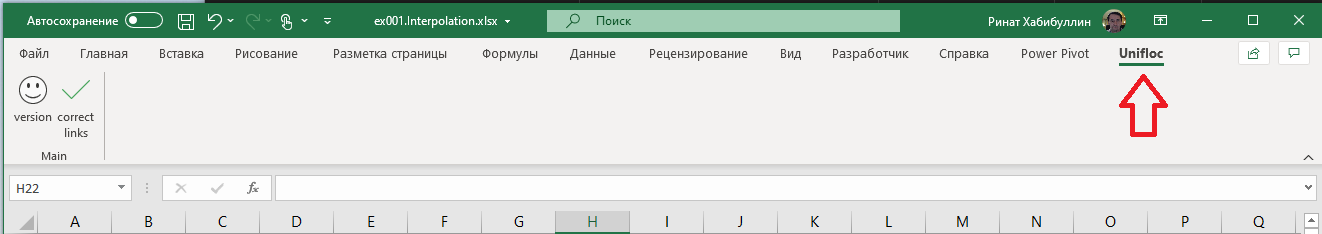
\includegraphics[width=0.8\linewidth]{excel_unifloc_tab}}
		\caption{Открытая панель Unifloc}
		\label{ris:excel_unifloc_tab}
	\end{figure}
	
	\item При необходимости вывести массив значений как результат расчета функций \mintinline{vb.net}{crv_solve} или \mintinline{vb.net}{crv_intersection} используйте комбинацию клавиш \texttt{Cntrl+Shift+Enter} или динамические массивы\footnote{подробнее про динамические массивы (dynamic arrays) можно посмотреть в интернете, например - https://www.planetaexcel.ru/techniques/2/9112/}(для новых версий Excel). Если для динамических массивов требуется подавить вывод массива - используйте знак @ в строке вызова, например как \mintinline{vb.net}{=@crv_solve(...)}.
	
	\item Все названия функций \unf{} начинаются с префикса. Это позволяет быстро искать необходимые функции. При запущенной надстройке достаточно начать вводить в ячейку формулу, например ввести \texttt{=PVT} как Excel откроет выпадающий список с подсказкой, показывающий возможные варианты названий функций (смотри рис. \ref{ris:Ex10_2}). 
	
	\begin{figure}[h!]
		\center{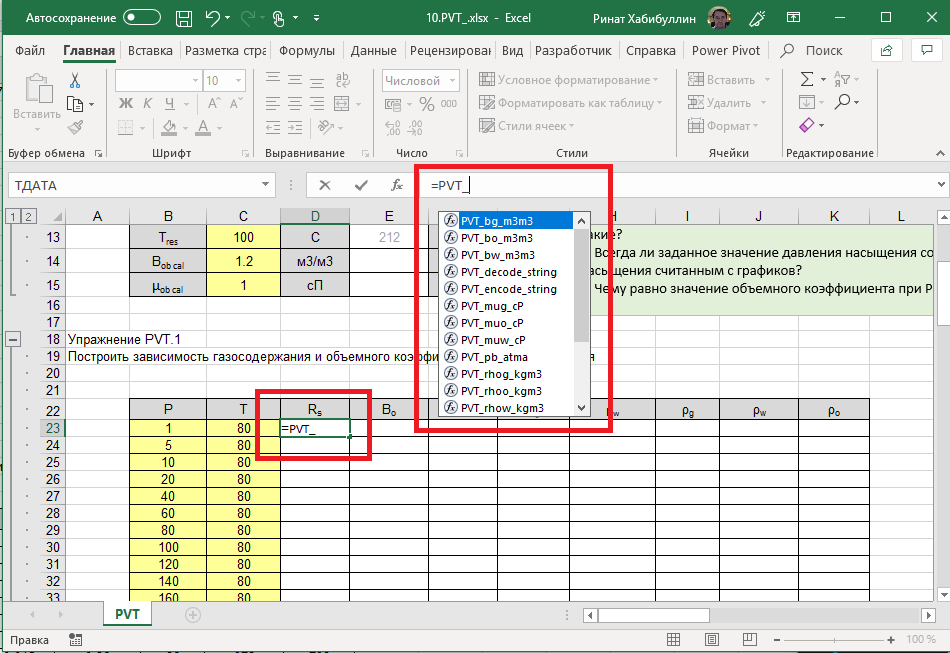
\includegraphics[width=0.8\linewidth]{Ex10_2}}
		\caption{Выпадающий список с подсказками названий функции}
		\label{ris:Ex10_2}
	\end{figure}
	
	\item 	Из выпадающего списка выберите функцию \texttt{=PVT\_Rs\_m3m3(} после чего нажмите кнопку $f_x$ "вставить функцию"  слева от строки формул. Это вызовет окно задания параметров функции, в котором будут указаны все параметры, которые необходимо ввести (смотри рис. \ref{ris:Ex10_3}). В этом окно можно задать необходимые значения параметров или указать ссылки на соответствующие ячейки. Для "хороших" функций в окне задания параметров функции будут подсказки. Также в окне задания параметров можно сразу видеть результат расчета если задан достаточный набор параметров.
	
	\begin{figure}[h!]
		\center{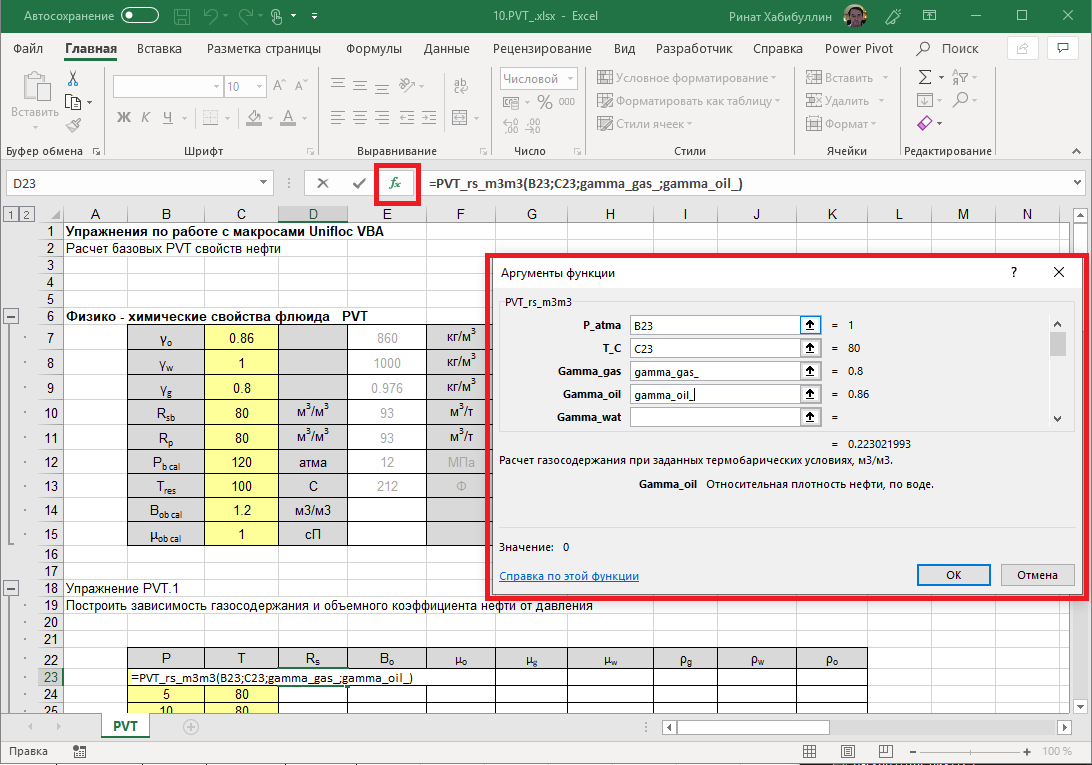
\includegraphics[width=0.8\linewidth]{Ex10_3}}
		\caption{Окно ввода аргументов функции}
		\label{ris:Ex10_3}
	\end{figure}
	
	\item После ввода всех параметров и нажатия кнопки ОК в ячейке должен отобразиться результат расчета. Воспользовавшись инструментом "Влияющие ячейки" на вкладке "Формулы"\ можно отследить на какие ячейки ссылается введенная формула (смотри рис. \ref{ris:Ex10_4})
	\begin{figure}[h!]
		\center{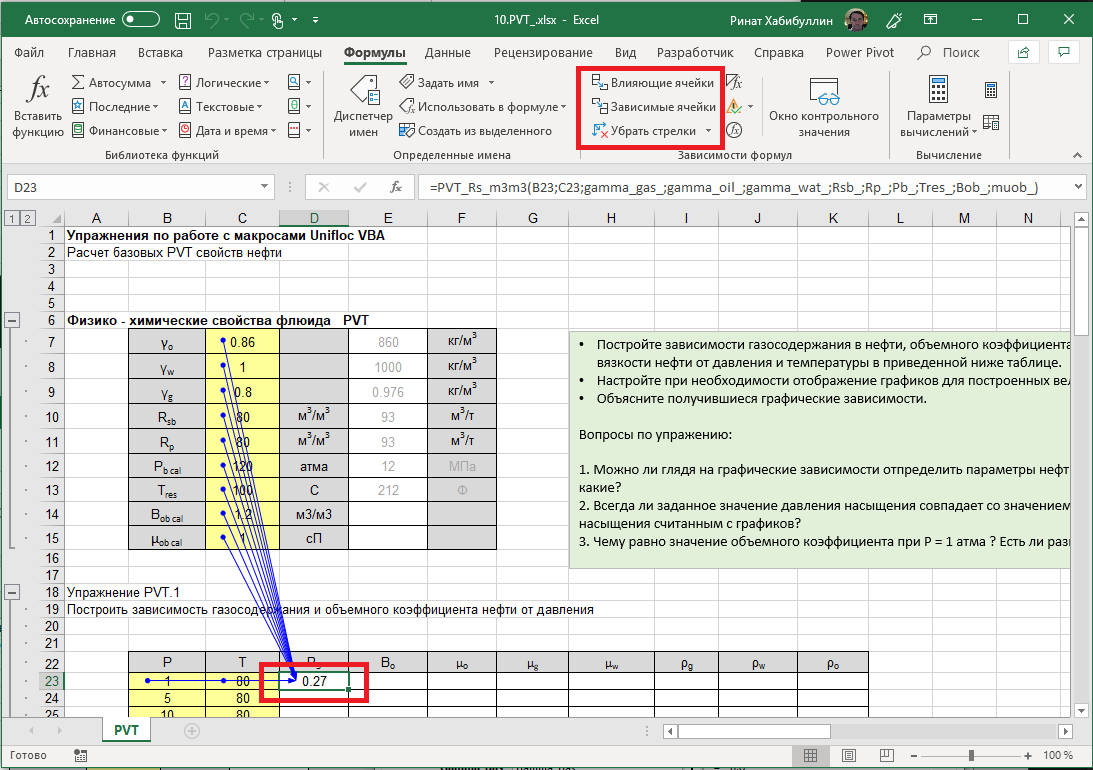
\includegraphics[width=0.8\linewidth]{Ex10_4}}
		\caption{Результат вызова пользовательской функции с отображение влияющих ячеек}
		\label{ris:Ex10_4}
	\end{figure}
\end{enumerate}


\section{Работа с таблично заданными кривыми}
Инженерный анализ требует умения ловко работать с графическими данными - кривыми, картами, кросс плотами и графиками. Кроме отображения графических данных, что легко делается стандартными программами - часто требует проводить по ним расчеты. Набор функций \unf{} для работы с таблично заданными кривыми может оказать полезными для этих целей. 

Функции \unf{} для работы с таблично заданными кривыми начинаются с префикса \mintinline{vb.net}{crv_}, от слова curve. Доступна функциональность
\begin{itemize}	
	\item интерполяции различными методами (работает и экстраполяция)
	\item поиска решения уравнения вида $f(x) = с$ где функция $f(x)$ задана таблицей (ищется решение для линейной аппроксимации)
	\item поиска пересечений двух кривых заданных таблицами (ищется решение для линейно аппроксимации)	
\end{itemize}
В коде можно обнаружить еще ряд функций, но они не будут описываться в данном руководстве, хотя по ним можно найти примеры в папке \texttt{examples} репозитория.

\subsection{Интерполяция линейная и сплайнами}
Файл примера \texttt{ex001.Interpolation.xlsx} можно найти в папке \texttt{exercises} репозитория \unf{}.

\begin{enumerate}
	\item Для работы с примером должна быть запущена надстройка \unf{}. Убедиться, что надстройка запущена можно найдя вкладку Unifloc в панели меню Excel, рис. \ref{ris:excel_unifloc_tab}.
	

	
	\item Откройте файл с упражнением \texttt{ex001.Interpolation.xlsx} (смотри рис. \ref{ris:Ex001_1}).
	
	\begin{figure}[h!]
		\center{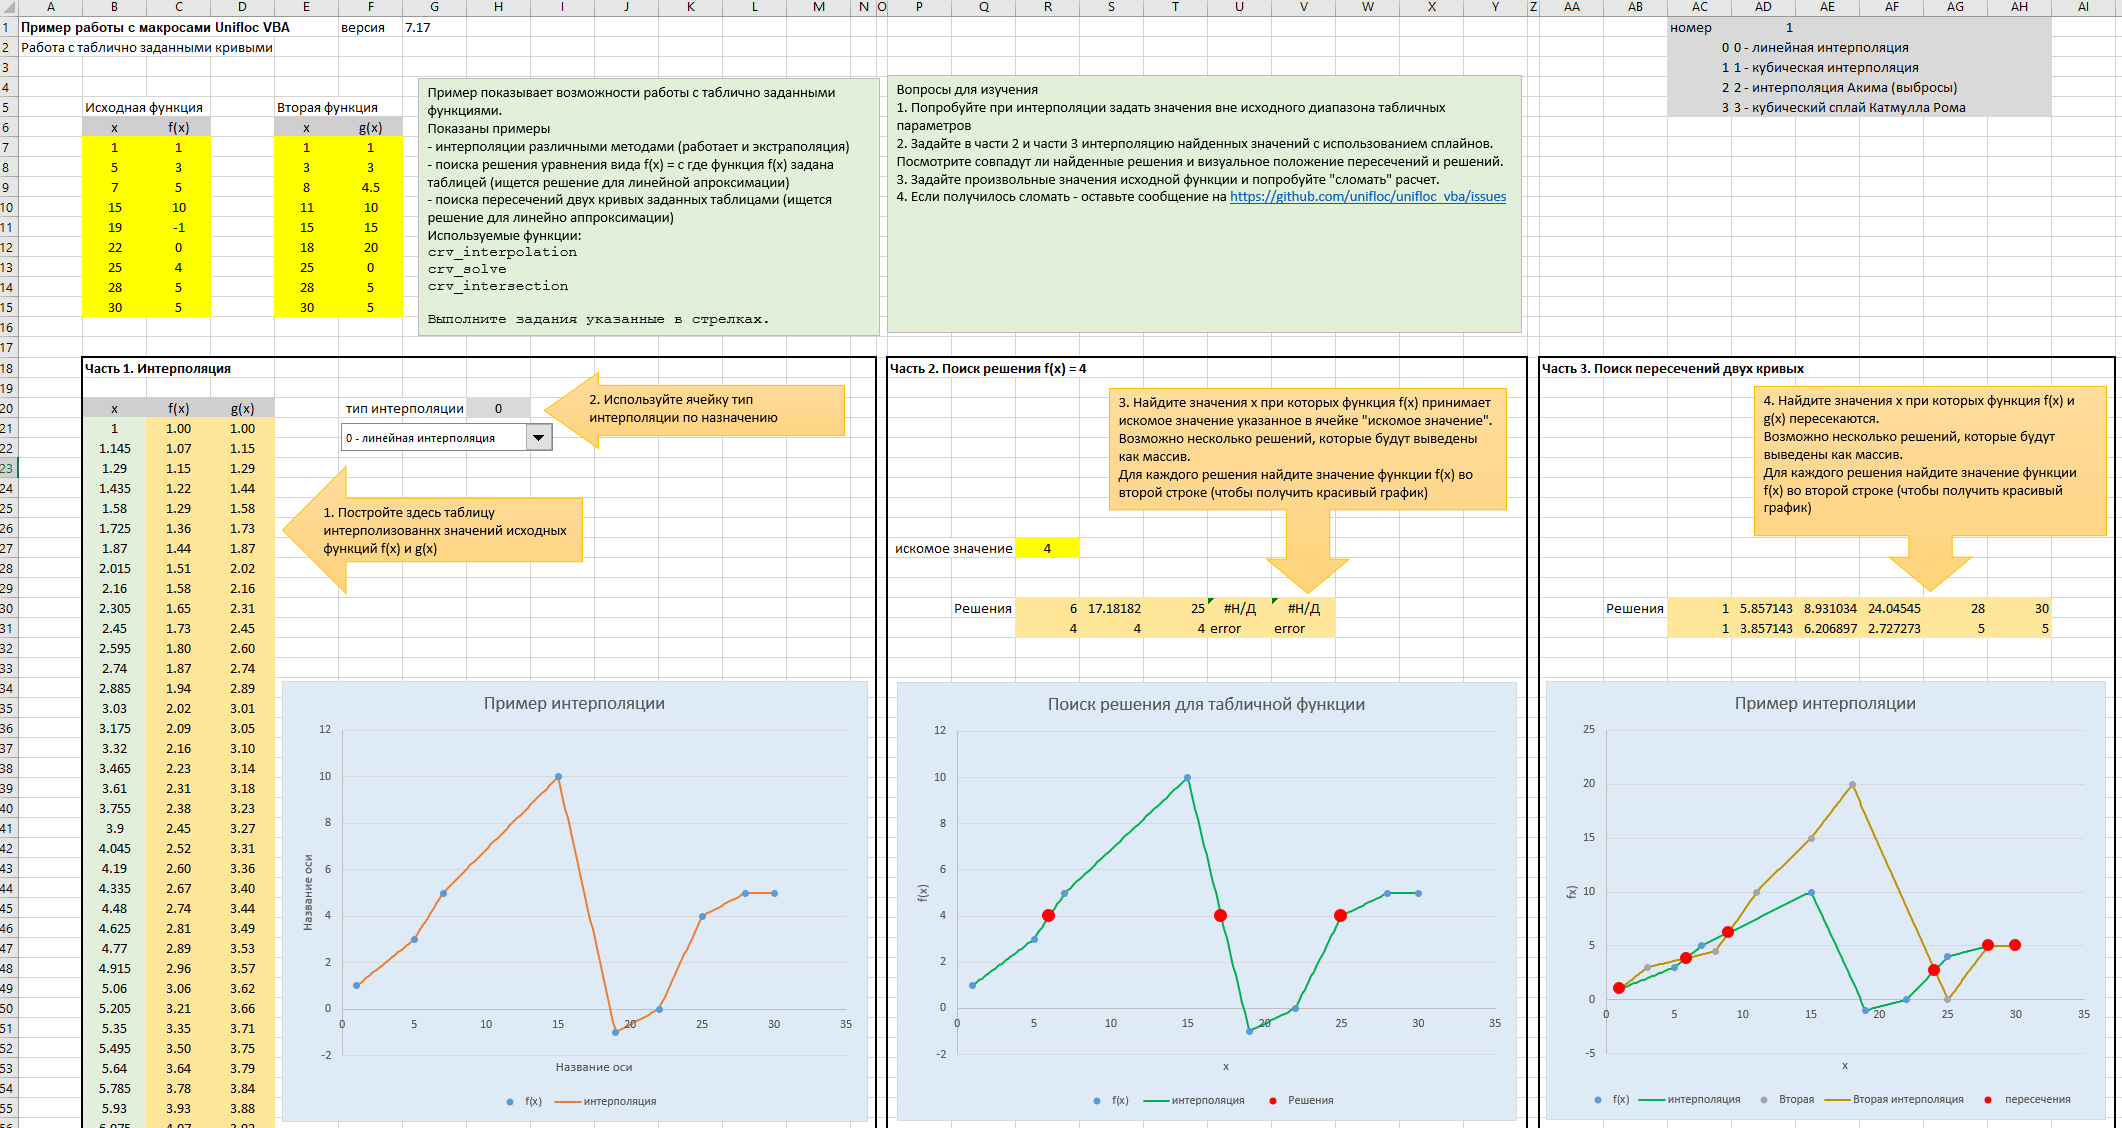
\includegraphics[width=1\linewidth]{Ex001_1}}
		\caption{Упражнение \texttt{ex001.Interpolation.xlsx} со всеми заполненными полями}
		\label{ris:Ex001_1}
	\end{figure}
	
	Пример разделен на три части: Часть 1. Интерполяция; Часть 2. Поиска решения $f(x)=c$; Часть 3.Поиск пересечения двух кривых.
	
	\item Выполните задания указанные в стрелках (последовательность выполнения по номерам стрелок). При этом должны автоматически построиться графики как на рисунке \ref{ris:Ex001_1}).
	

	
	\item Постарайтесь ответить на вопросы в блоке "Вопросы для изучения"

\end{enumerate}

\section{Расчет базовых PVT свойств флюидов}

Расчет физико химических свойств пластовых флюидов (PVT параметров) лежит в основе всех расчетов систем нефтедобычи. При решении прикладных задач редко возникает необходимость расчета PVT свойств непосредственно, однако понимание принципа их расчета, а особенно зависимости результатов расчета от исходных данных важно.
   
Для выполнения упражнения используйте файл "ex010.PVT.xlsx"

\begin{enumerate}

	\item Откройте файл с упражнением \texttt{10.PVT.xlsx} (смотри рис. \ref{ris:Ex10_1}).
	
	\begin{figure}[h!]
		\center{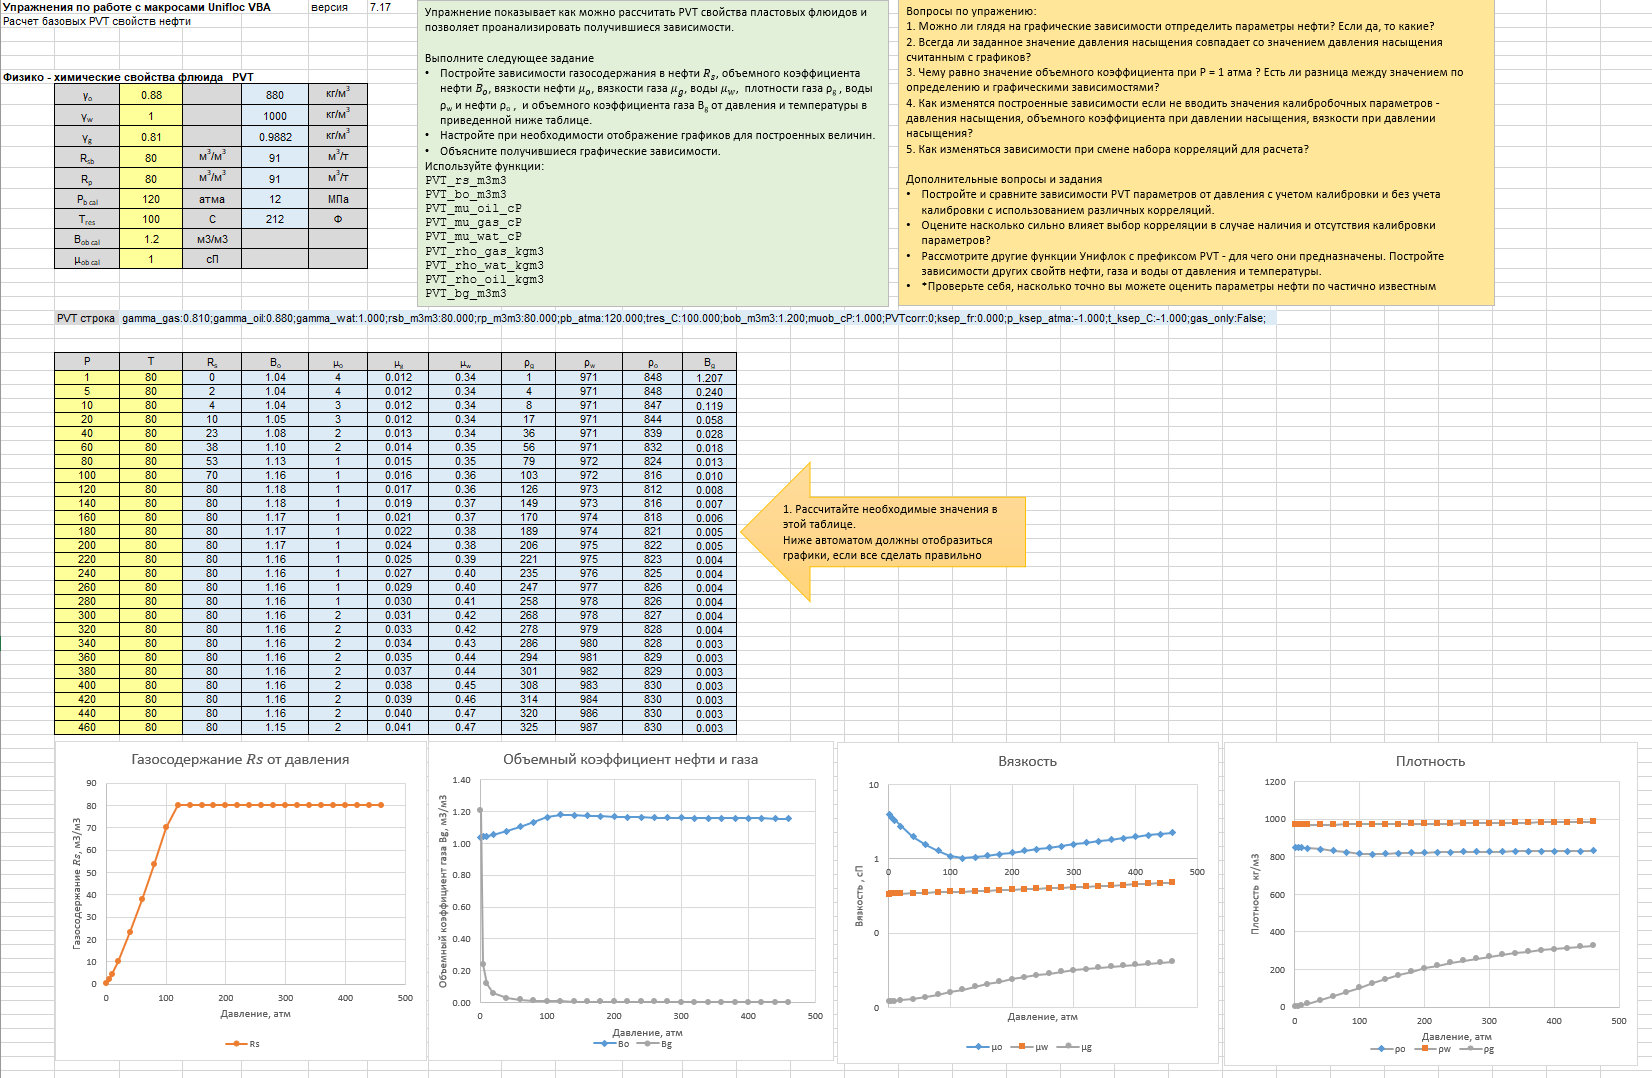
\includegraphics[width=1\linewidth]{Ex10_1}}
		\caption{Упражнение \texttt{ex010.PVT.xlsx} со всеми заполненными полями.}
		\label{ris:Ex10_1}
	\end{figure}
	
	\item Выполните задания указанные в описании. Задания просты -- требуется рассчитать таблицу значений для построения графиков и провести анализ построенных графиков. Названия необходимых функций указаны в описании  \ref{ris:Ex10_1}). Вопросы по упражнению помогут вам провести анализ. Текст заданий не приводится в описании, так как файлы упражнений первичны. Любые изменения скорее будут вноситься в файлы с заданиями, нежели в описание.
	
	\item Ответьте на вопросы по упражнению приведенные в рабочей книге.
	 
\end{enumerate}

\section{Расчет свойств потока флюидов}

PVT функции описывают свойства флюидов. Можно представить себе, что они описывают свойства флюидов находящихся в PVT бомбе - устройстве для отбора проб. В этом случае флюиды неподвижны и находятся в равновесном состоянии. На практике приходится иметь дело с флюидами двигающимися в скважине или трубопроводе - с потоком флюидов. В потоке флюидов добавляются дополнительные параметры -- расход флюидов или дебит $Q_{liq}, Q_g$ и обводненность $f_w$ -- показатель показывающий объемную долю воды в потоке. 
Функции работающие с потоками в \unf{} имеют префикс \mintinline{vb.net}{MF_}. Префикс должен намекать на многофазность потока и на самом деле плох с лингвистической точки зрения (multiphase - has no F letter), но удобен с программистской точки зрения и уже поздно его менять.

Файл примера \mintinline{vb.net}{ex011.Gas_fraction.xlsx} можно найти в папке \texttt{exercises} репозитория \unf{}.

\begin{enumerate}
	
	\item Откройте файл с упражнением \texttt{10.PVT.xlsx} (смотри рис. \ref{ris:Ex11_1}).
	
	\begin{figure}[h!]
		\center{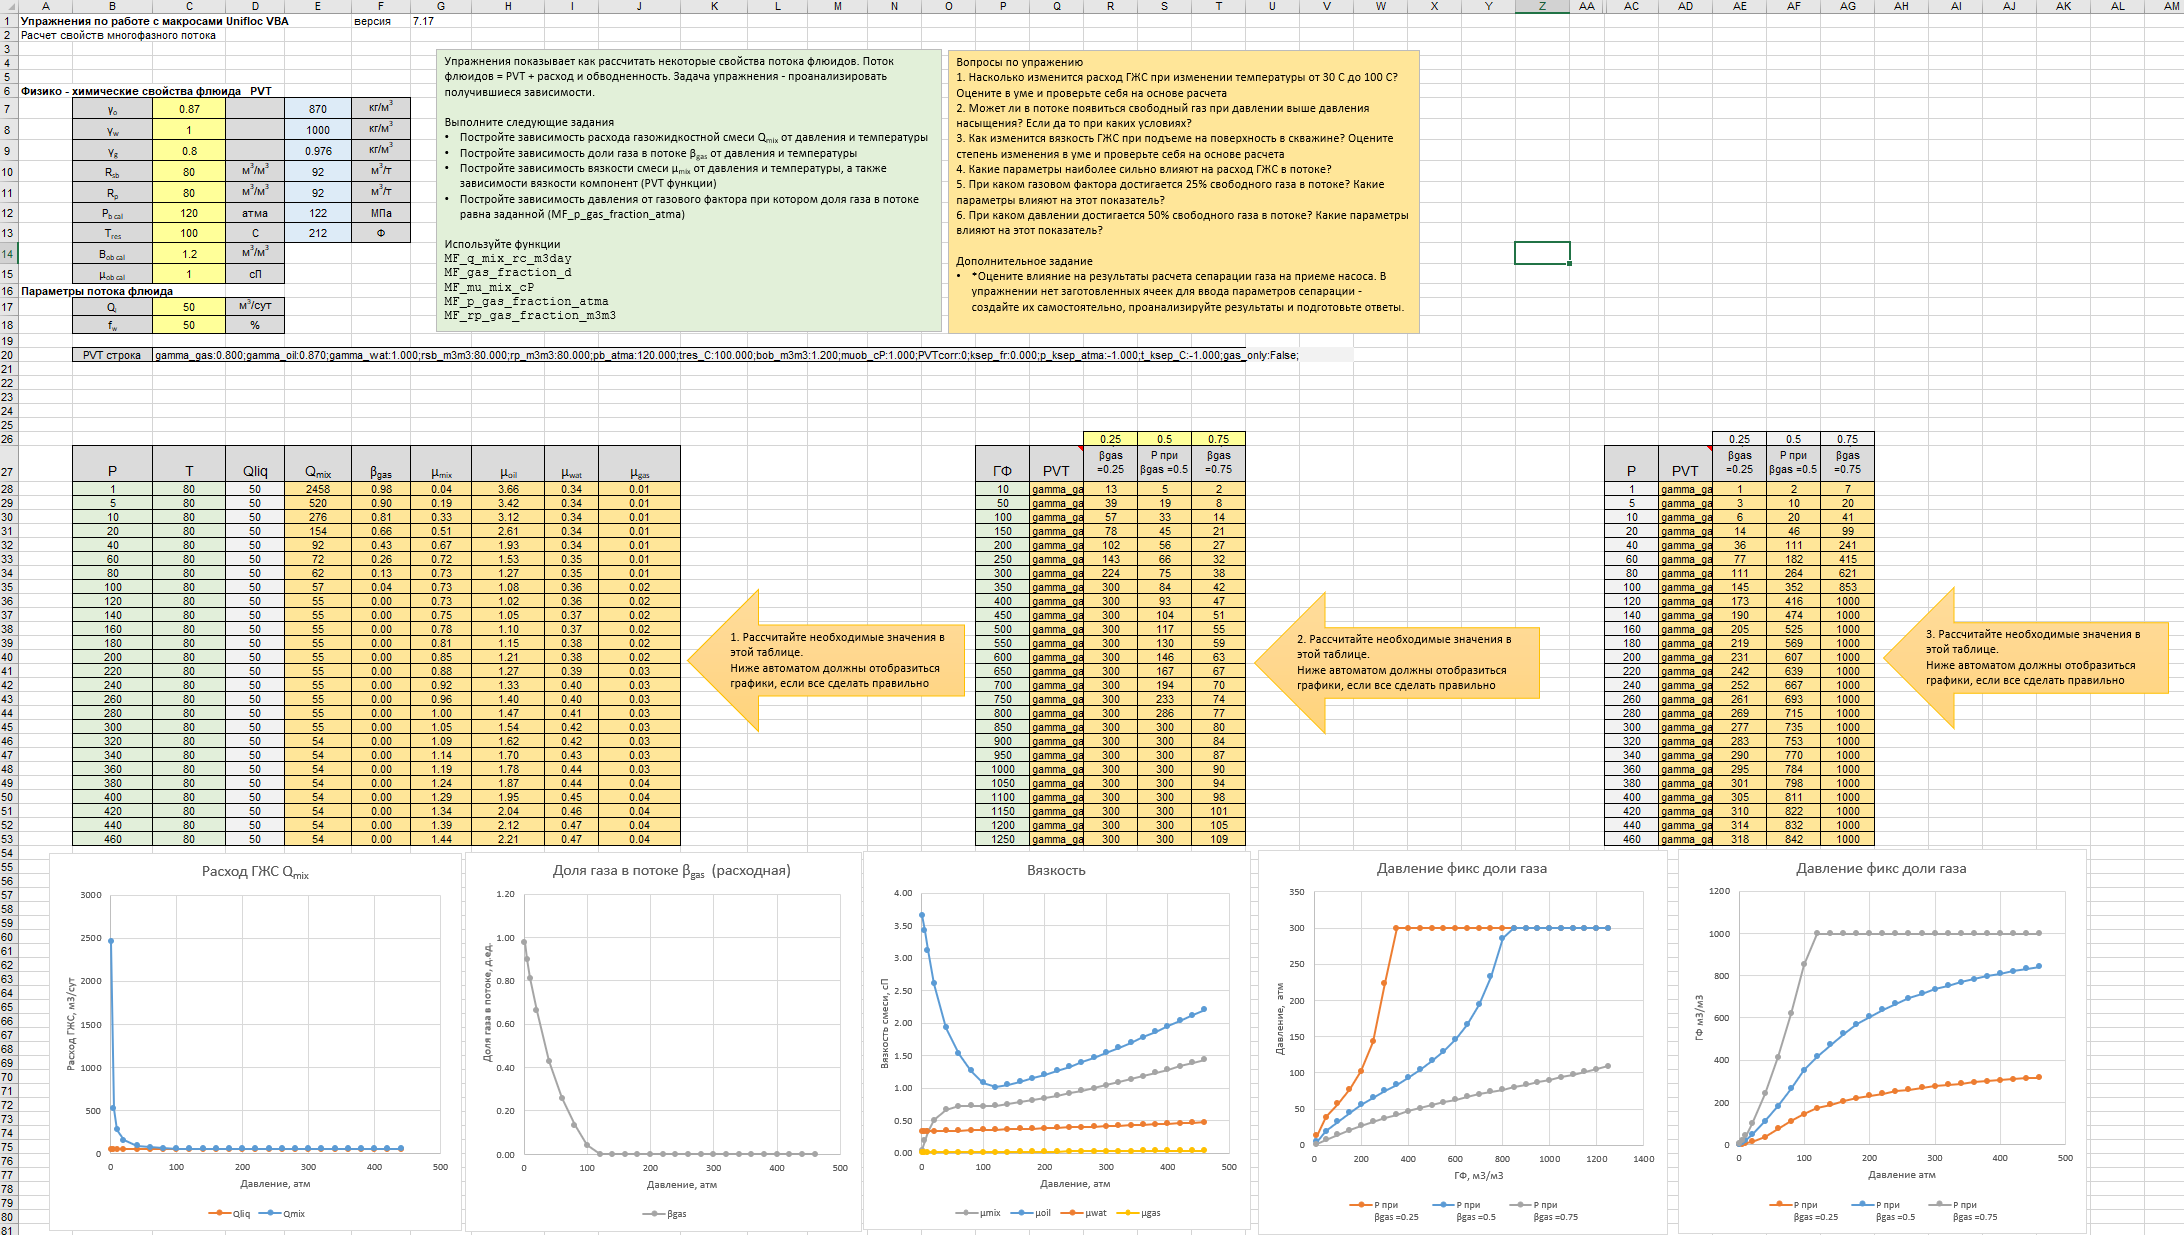
\includegraphics[width=1\linewidth]{Ex11_1}}
		\caption{Упражнение \mintinline{vb.net}{ex011.Gas_fraction.xlsx} со всеми заполненными полями }
		\label{ris:Ex11_1}
	\end{figure}
	
	\item Выполните задания указанные в описании. Задания просты -- требуется рассчитать три таблицы значений для построения графиков и провести анализ построенных графиков. Названия необходимых функций указаны в описании  \ref{ris:Ex11_1}). Вопросы по упражнению помогут вам провести анализ. Текст заданий не приводится в описании, так как файлы упражнений первичны. Любые изменения скорее будут вноситься в файлы с заданиями, нежели в описание.
	
	\item Ответьте на вопросы по упражнению приведенные в рабочей книге.
	
	\item Выполните дополнительное задание, если чувствуете силы. В дополнительном задании говорится о сепарации газа на приеме насоса. Имеется в виду следующее - если у нас есть пластовые флюиды, свойства которых мы знаем и можем задать, то после сепарации части свободного газа, что часто происходит на скважинном насосе, свойства флюида изменятся. Изменится его эффективное давление насыщения (потому что мы убрали часть газа) и газосодержание при давлении насыщения. И соответственно поплывут и остальные свойства. Это можно учесть задав в \mintinline{vb.net}{PVT_Encode()} три параметра - коэффициент сепарации газа $K_{sep}$, давление при которой произошла сепарации $P_{sep}$ и температуру при которой произошла сепарация $T_{sep}$. Подробнее про это можно найти в соответствующих разделах (поэтому тут это задание дополнительное).
	
\end{enumerate}

\section{Расчет производительности скважины}

Стационарная модель притока к скважине (закон Дарси с поправкой Вогеля) - одна из самых простых и распространенных моделей, широко применяемая в индустрии. \unf{} содержит функции позволяющие упростить расчет индикаторной кривой. Такие функции имеют префикс \mintinline{vb.net}{IPR_} от Inflow Performance Relationship.

Файл примера \mintinline{vb.net}{ex020.IPR.xlsx} можно найти в папке \texttt{exercises} репозитория \unf{}.

\begin{enumerate}
	
	\item Откройте файл с упражнением \texttt{ex020.IPR.xlsx} (смотри рис. \ref{ris:Ex20_1}).
	
		\begin{figure}[h!]
			\center{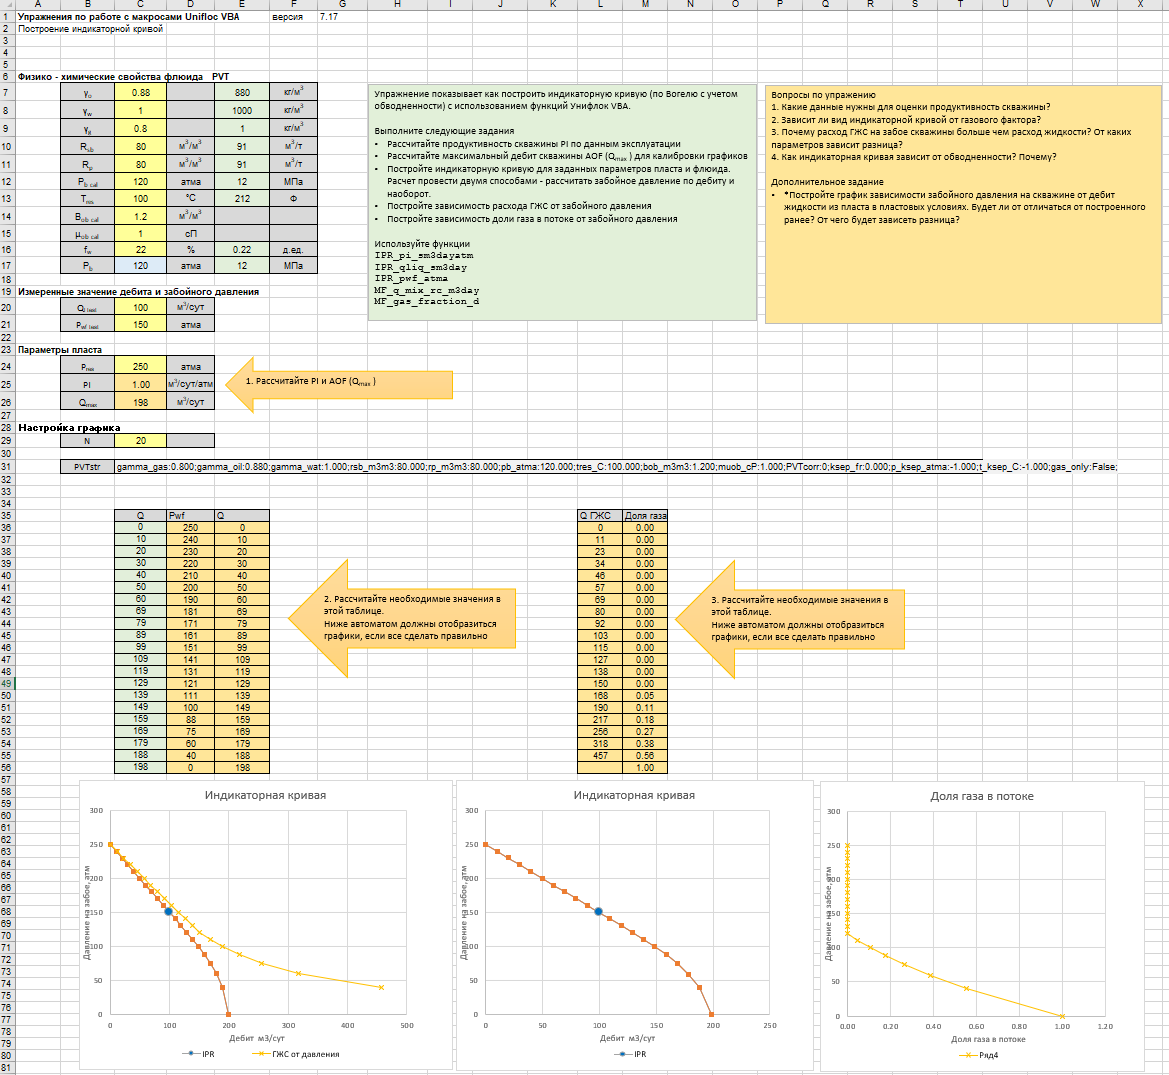
\includegraphics[width=1\linewidth]{Ex20_1}}
			\caption{Упражнение \mintinline{vb.net}{ex020.IPR.xlsx} со всеми заполненными полями }
			\label{ris:Ex20_1}
		\end{figure}

	\item Выполните задания указанные в описании. Задания просты -- требуется рассчитать три таблицы значений для построения графиков и провести анализ построенных графиков. Названия необходимых функций указаны в описании  \ref{ris:Ex11_1}). Вопросы по упражнению помогут вам провести анализ. Текст заданий не приводится в описании, так как файлы упражнений первичны. Любые изменения скорее будут вноситься в файлы с заданиями, нежели в описание.
	
	\item Ответьте на вопросы по упражнению приведенные в рабочей книге.
	
	\item Выполните дополнительное задание, если чувствуете силы.

\end{enumerate}

Коэффициент продуктивности $PI$ скважины рассчитывается в ячейке С25 по замеренным данным  с помощью функции

{ \small  \texttt{=IPR\_PI\_sm3dayatm(qltest\_;Pwftest\_;Pres\_;fw\_;Pb\_)}}

А максимальный дебит $Q_{max}$ при максимальной депрессии с забойным давлением равным нулю

{ \small  \texttt{=IPR\_Qliq\_sm3Day(PI\_;Pres\_;0;fw\_;Pb\_)}}




\section{Расчет штуцера}

Для контроля дебита и/или давления на добывающих скважинах вблизи устья может устанавливаться штуцер. Для штуцера, как для любого гидравлического элемента, возможно 4 варианта расчета - расчет давления по потоку, расчет давления против потока, расчет потока по давлениям и настройка модели штуцера по известным давлениям и потоку. В упражнении демонстрируются все варианты расчета. 

Файл примера \mintinline{vb.net}{ex040.MF_choke.xlsx} можно найти в папке \texttt{exercises} репозитория \unf{}.

\begin{enumerate}
	
	\item Откройте файл с упражнением \mintinline{vb.net}{ex040.MF_choke.xlsx} (смотри рис.\ref{ris:Ex40_1}).
	
	\begin{figure}[h!]
		\center{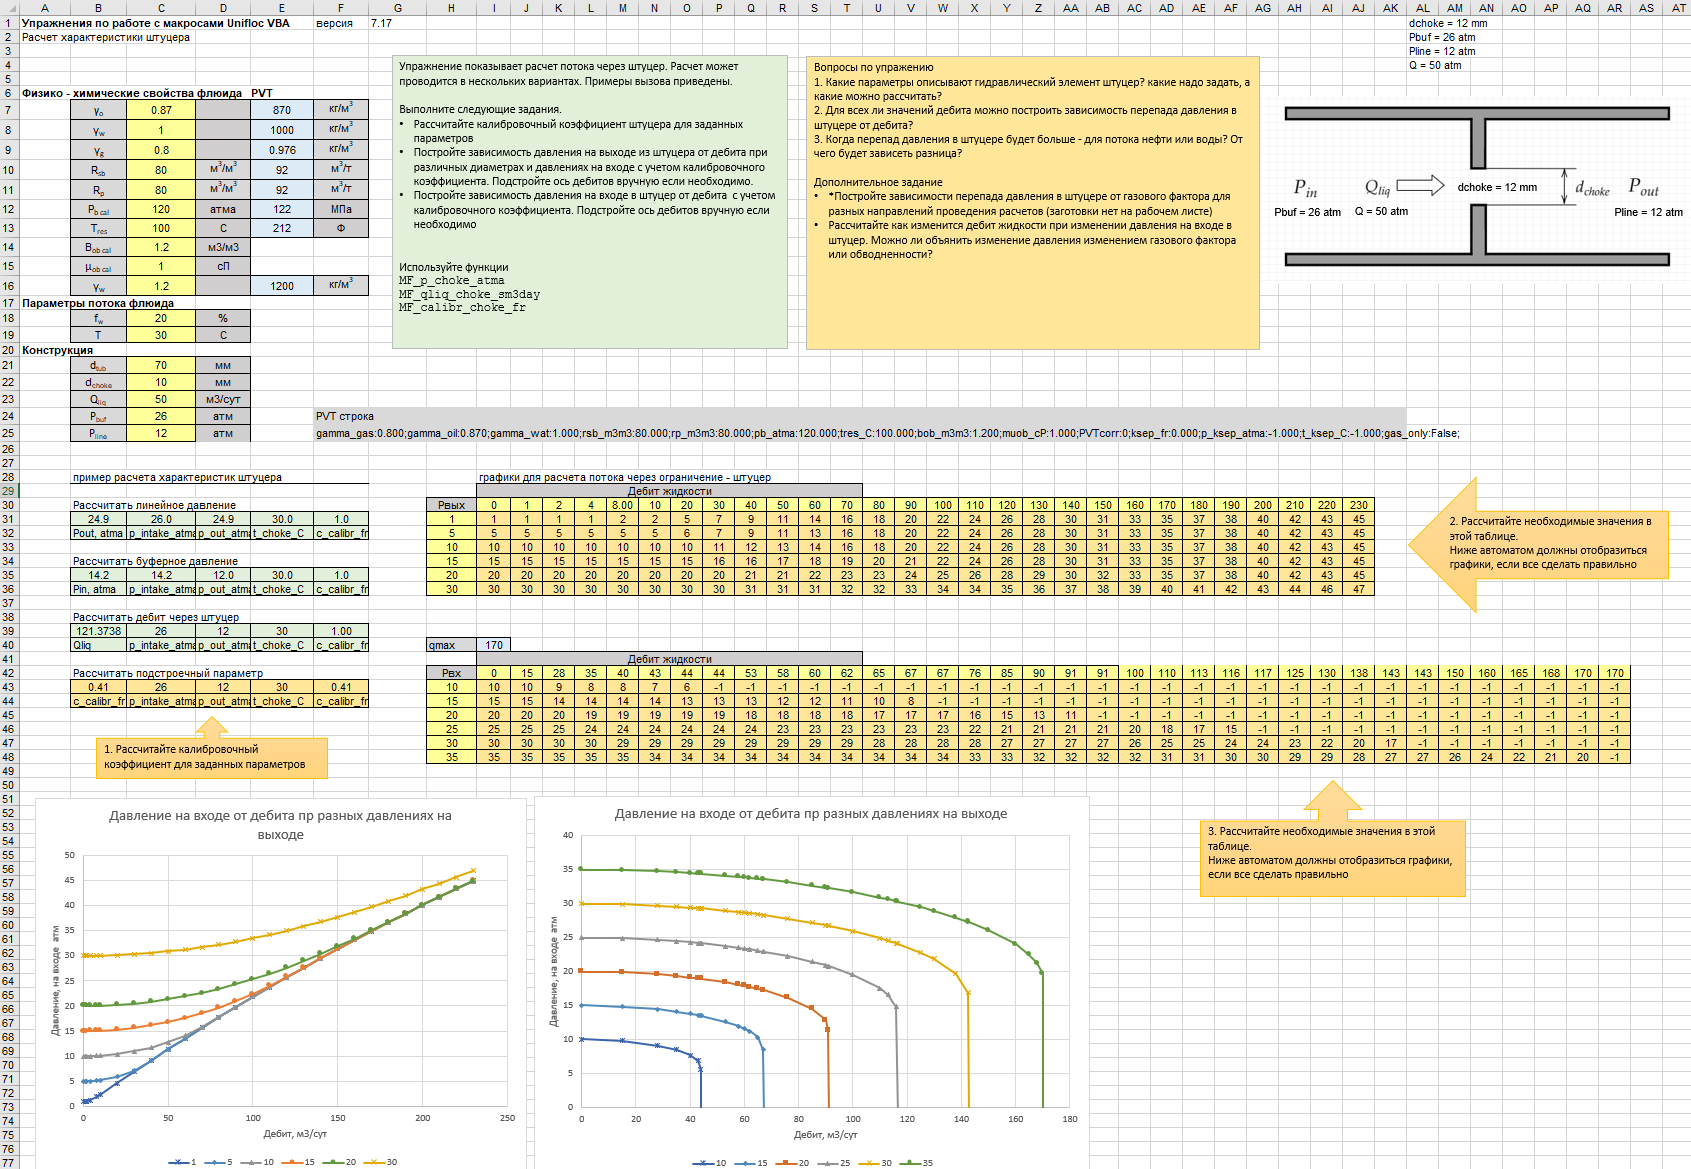
\includegraphics[width=1\linewidth]{Ex40_1}}
		\caption{Упражнение \mintinline{vb.net}{ex040.MF_choke.xlsx} со всеми заполненными полями }
		\label{ris:Ex40_1}
	\end{figure}
	
	\item Выполните задания указанные в описании. Названия необходимых функций указаны в описании  \ref{ris:Ex11_1}). При построении графиков может потребоваться изменить значения дебитов по которым проводится расчет для корректного отображения графиков. Текст заданий не приводится в описании, так как файлы упражнений первичны. Любые изменения скорее будут вноситься в файлы с заданиями, нежели в описание. 
	
	\item Ответьте на вопросы по упражнению приведенные в рабочей книге.
	
	\item Выполните дополнительное задание, если чувствуете силы.
	
\end{enumerate}


\section{Расчет распределения давления в трубе}
Расчет многофазных потоков в трубе - ключевой для анализа работы скважин и скважинного оборудования. Под расчетов трубы подразумевается в первую очередь расчет распределения давления. Иногда требуется рассчитать и распределение температуры. 
На распределение давления в трубе среди прочих параметров влияют режим потока газожидкостной смеси и явление проскальзывание газа. Недоучет данных параметров может привести к значительным ошибкам. Методы для расчета распределения давления можно разделить на две категории: корреляции, полученные экспериментальным путем и механистические модели, в основе которых заложены физические модели.

В \unf{} есть два набора функций для работы с трубой - простые по работе с прямым участком трубы \mintinline{vb.net}{MF_p_pipe} и более сложные по работе с участком трубопровода с учетом рельефа или инклинометрии \mintinline{vb.net}{MF_p_pipeline}

\subsection{Расчет прямолинейного участка трубы. Простой вариант}
Файл примера \mintinline{vb.net}{ex050.MF_pipe.xlsx} можно найти в папке \texttt{exercises} репозитория \unf{}.

\begin{enumerate}
	
	\item Откройте файл с упражнением \mintinline{vb.net}{ex050.MF_pipe.xlsx} (смотри рис.\ref{ris:Ex50_1}).
	
	\begin{figure}[h!]
		\center{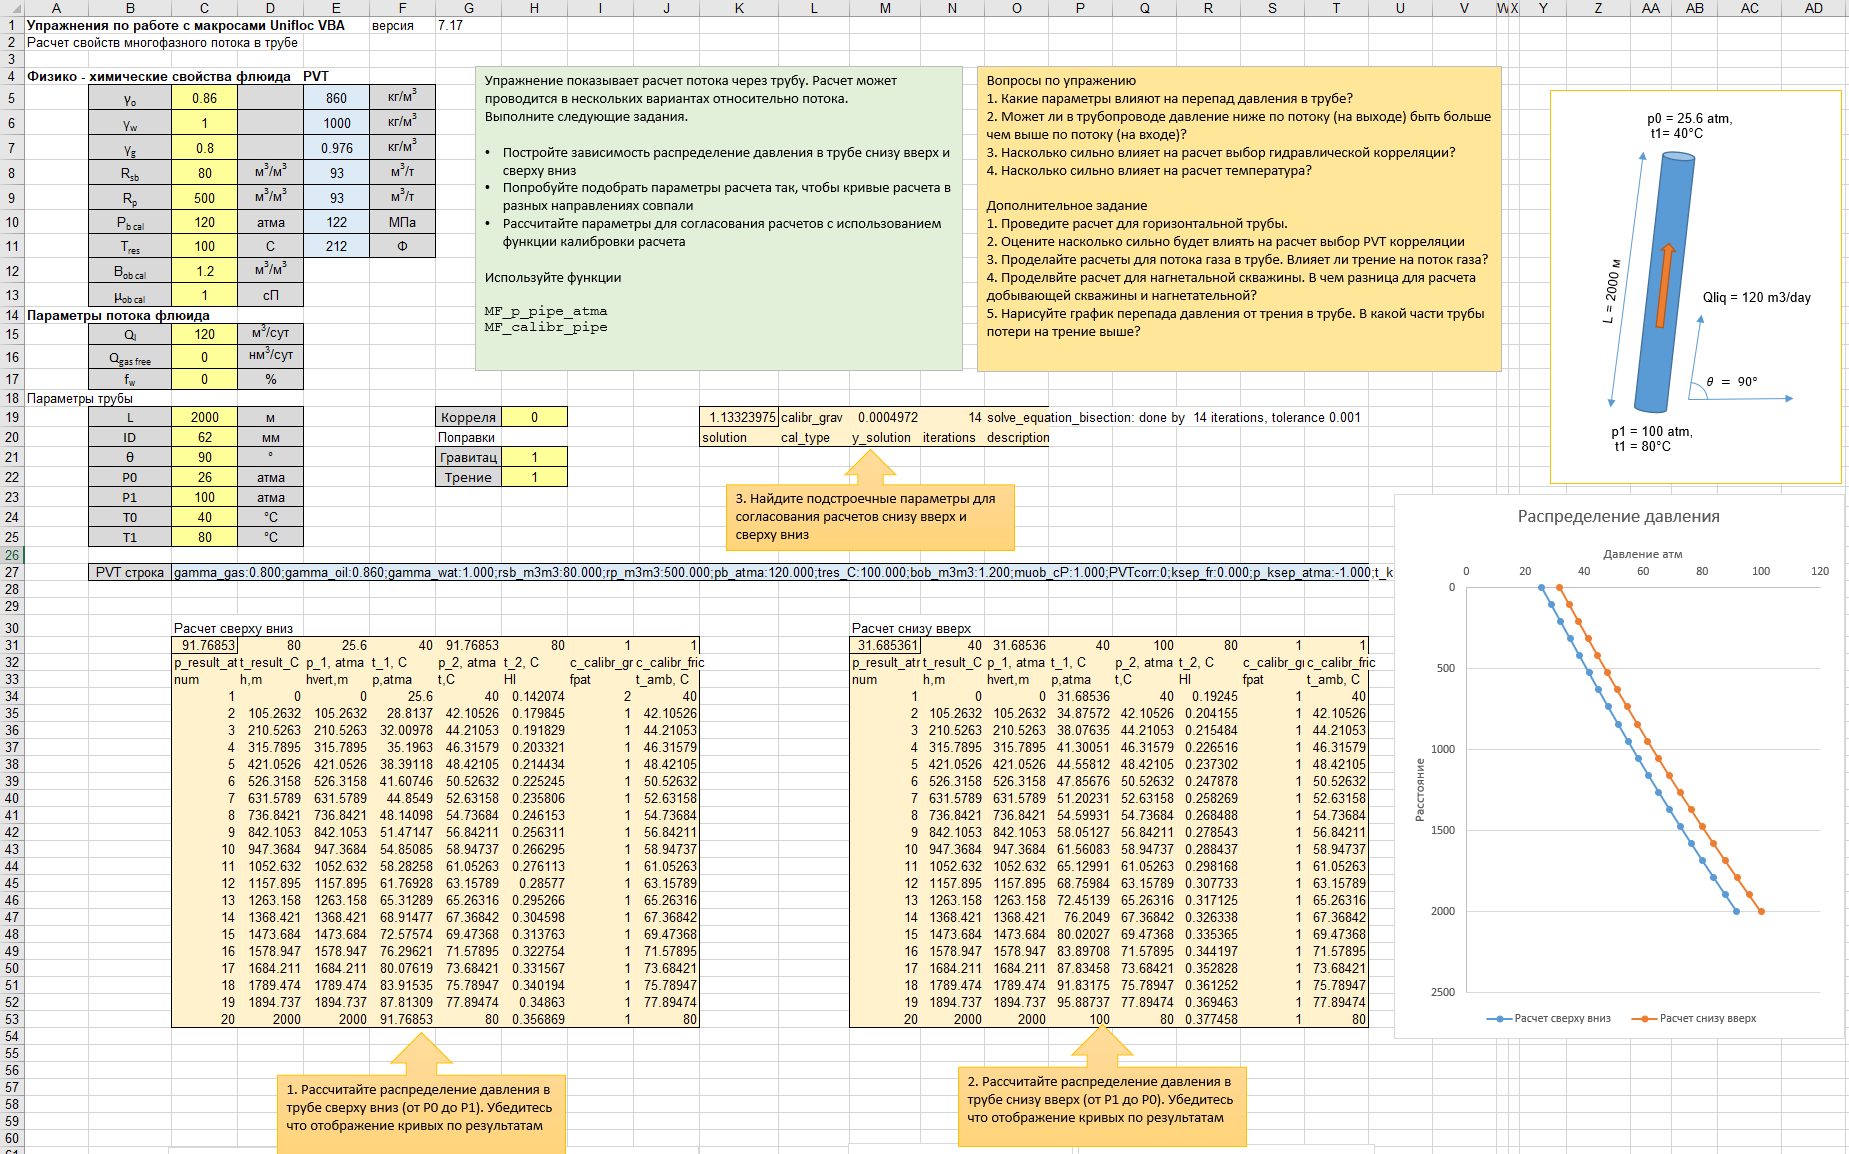
\includegraphics[width=1\linewidth]{Ex50_1}}
		\caption{Упражнение \mintinline{vb.net}{ex050.MF_pipe.xlsx} со всеми заполненными полями }
		\label{ris:Ex50_1}
	\end{figure}
	
	\item Выполните задания указанные в описании. Названия необходимых функций указаны в описании  \ref{ris:Ex50_1}). Текст заданий не приводится в описании, так как файлы упражнений первичны. Любые изменения скорее будут вноситься в файлы с заданиями, нежели в описание. 
	
	\item Ответьте на вопросы по упражнению приведенные в рабочей книге.
	
	\item Выполните дополнительное задание, если чувствуете силы.
	
\end{enumerate}





\section{Расчет коэффициентов сепарации}

Процессы сепарации на приеме погружного оборудования значительно влияют на процесс добычи. Как при естественной, так и при искусственной сепарации (при применении газосепараторов) меняются свойства многофазного потока, уменьшается газлифтный эффект, изменяется режим работы центробежного насоса.

В данном упражнении помимо стандартного определения PVT свойств требуется задать термобарические условия на приеме погружного оборудования (в месте, где происходит сепарация) и конструктивные параметры


\begin{figure}[h!]
	\center{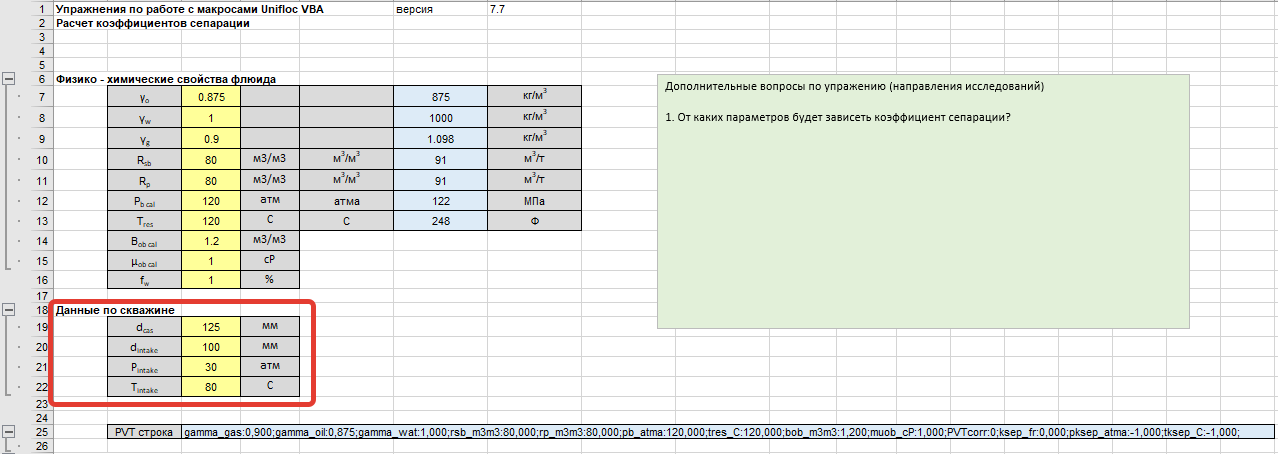
\includegraphics[width=1\linewidth]{Ex60_1}}
	\caption{Исходные данные для сепарации}
	\label{ris:Ex60_1}
\end{figure}

где

$d_{cas}$ - диаметр обсадной колонны, мм

$d_{intake}$ - диаметр приема погружного оборудования, мм

$P_{intake}$ - давление на приеме, атм

$T_{intake}$ - температура на приеме, С

Для вычисления коэффициента естественной сепарации в зависимости от дебита вставьте в ячейку E32 следующую формулу 

{ \small  \texttt{=MF\_ksep\_natural\_d(C32; wc\_; Pintake\_; Tintake\_; Dintake\_; Dcas\_; PVT\_str\_)}}

Для проведения экспериментов по влиянию изменения диаметра обсадной колонны воспользуйтесь в ячейке F32 формулой

{ \small  \texttt{=MF\_ksep\_natural\_d(C32; wc\_; Pintake\_; Tintake\_; Dintake\_; Dcas\_*cf\_dcas\_; PVT\_str\_)}}

При этом в ячейке F30 с помощью коэффициента Вы можете варьировать диаметр обсадной колонны

Для расчета доли газа в газосепараторе применяется функция

{ \small  \texttt{=MF\_gas\_fraction\_d(Pintake\_;Tintake\_;0;PVT\_str\_)*(1-F32)
}}

Коэффициент сепарации газосепаратора

{ \small  \texttt{=MF\_ksep\_gasseparator\_d(gassep\_type;G32;C32)
}}

При этом можно менять тип газосепаратора в ячейке H30

Общий коэффициент сепарации

{ \small  \texttt{=MF\_ksep\_total\_d(E32;H32)
}}

\begin{figure}[h!]
	\center{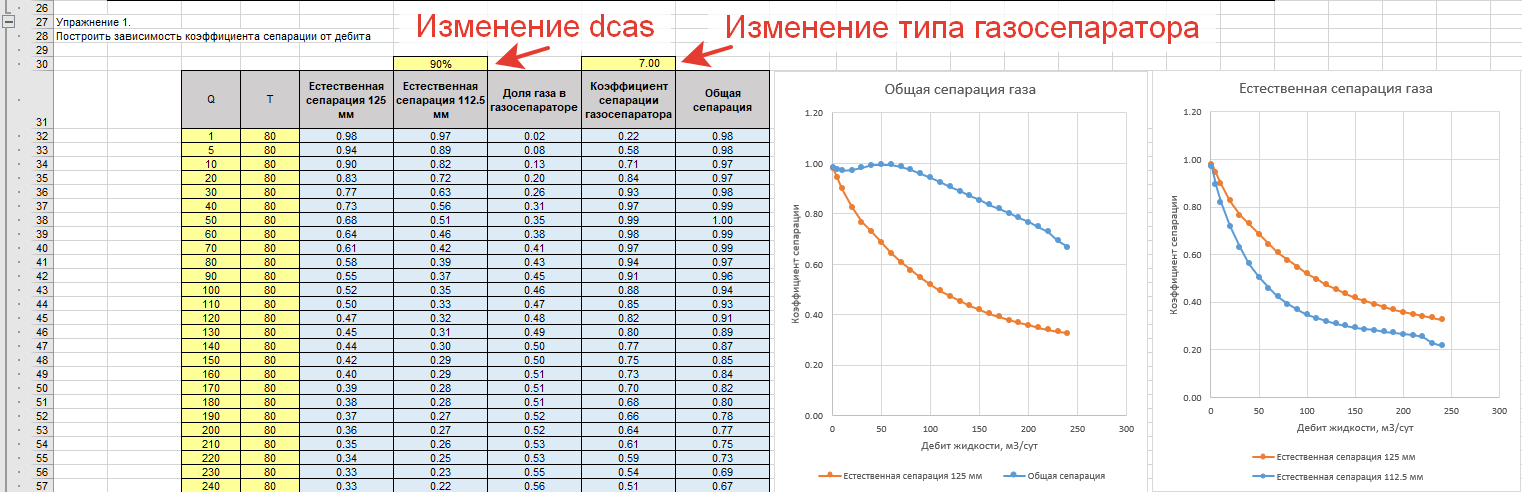
\includegraphics[width=1\linewidth]{Ex60_2}}
	\caption{Результаты расчета естественной и искусственной сепарации}
	\label{ris:Ex60_2}
\end{figure}

Вопросы к упражнению

\begin{enumerate}
	\item От каких параметров будет зависеть коэффициент сепарации?
	\item Как взаимосвязана естественная и искусственная сепарация? 
\end{enumerate}


\section{Анализ работы ЭЦН}

Сегодня доминирующая доля нефти в РФ добывается при помощи ЭЦН. Требуется детальное понимание основных особенностях эксплуатации данного оборудования, режимах работы, возможных осложнениях по причине высокой вязкости продукции, газосодержания, механических примесей и т.д.

Наиболее ценную информацию о работе насоса может дать его характеристика: зависимость параметров работы ЭЦН - напора, потребляемой мощности, перепада давления, КПД, от подачи (дебита скважины)

Для анализа работы скважины, оснащенной УЭЦН, требуются следующие исходные данные

\begin{enumerate}
	\item Физико - химические свойства флюида
	\item Данные по скважине
	\item Данные по ЭЦН
	\item Параметры пласта
\end{enumerate}

PVT свойства задаются аналогично предыдущим упражнениям, а для параметров, характеризующих скважину, приняты следующие обозначения

$H_{mes}$ - глубина скважины измеренная (вдоль ствола скважины), м

$H_{mes}- H_{vert}$ - удлинение ствола скважины, м

$H_{pump}$ - глубина спуска насоса, м

$ID_{cas}$ - внутренний диаметр обсадной колонны, мм

$OD_{tub}$ - внешний диаметр НКТ, мм

$ID_{tub}$ - внутренний диаметр НКТ, мм

$D_{intake}$ - диаметр приемной сетки ЭЦН, мм

$P_{buf}$ - буферное давление, атм

$P_{intake}$ - давление на приеме ЭЦН, атм

$T_{intake}$ - температура на приеме ЭЦН, С

$P_{dis}$ - давление на выкиде ЭЦН, атм

$P_{wf}$ - давление на забое, атм

$Q_{liq}$ - дебит жидкости в поверхностных условиях, м3/сут

$f_w$ - обводненность в поверхностных условиях, \%

\begin{figure}[h!]
	\center{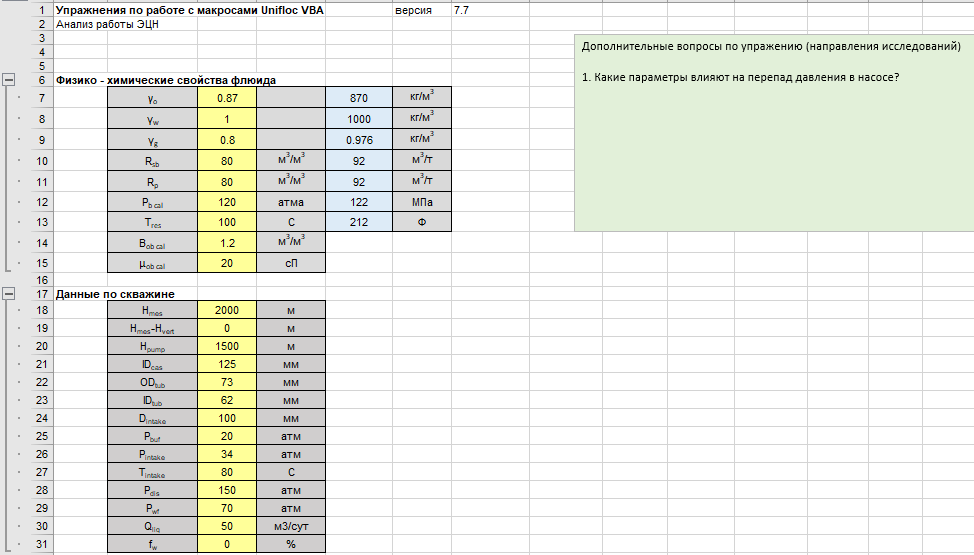
\includegraphics[width=1\linewidth]{Ex70_1}}
	\caption{Исходные данные для свойств флюида и параметров скважины}
	\label{ris:Ex70_1}
\end{figure}

Параметры, описывающие ЭЦН: 

ЭЦН $Q_{nom}$ - номинальная подача ЭЦН, м3/сут

ЭЦН $H_{nom}$ - номинальная напом ЭЦН, м

$F$ - частота питающего тока двигателя, Гц

ЭЦН $ID$ - идентификационный номер насоса (по формуле, см. ниже), находящийся в базе \unf

ЭЦН имя - обозначение насоса: название, габарит и номинальная подача (по формуле, см. ниже)

ЭЦН $Q_{max}$ - максимальная производительность насоса (по формуле, см. ниже), м3/сут

Ступени - количество ступеней, исходя из общего напора ЭЦН и напора одной ступени (по формуле, см. ниже), шт

$K_{sep_ГС}$ - коэффициент сепарации газосепаратора, \%

$P_{sep}$ - давление сепарации, атм

$T_{sep}$ - температура сепарации, С

Данные о пласте:

$P_{res}$ - пластовое давление, атм

$PI$ - коэффициент продуктивности скважины (по формуле, см. выше в упражнении IPR), м3/сут/атм

$\frac{dT}{dL}$ - геотермический градиент, град / 100 м

\begin{figure}[h!]
	\center{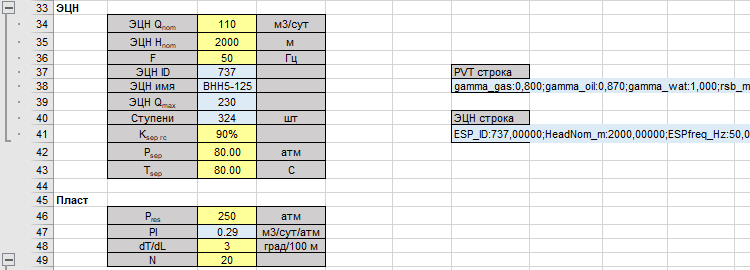
\includegraphics[width=1\linewidth]{Ex70_2}}
	\caption{Исходные данные для ЭЦН и пласта}
	\label{ris:Ex70_2}
\end{figure}

Для получения идентификационного номера насоса в базе \unf \ была использована формула

{ \small  \texttt{=ESP\_id\_by\_rate(Q\_ESP\_)}}

Для определения обозначения ЭЦН

{ \small  \texttt{=ESP\_name(C37)}}

Расчет максимально возможного дебита

{ \small  \texttt{=esp\_max\_rate\_m3day(Freq\_;PumpID\_)*1}}

Количество ступеней

{ \small  \texttt{=ЦЕЛОЕ(Head\_ESP\_/ESP\_head\_m(Q\_ESP\_;1;;PumpID\_))
}}

Также для удобства использования параметры насоса: ID, напор и рабочая частота, зашифровываются в строку с помощью функции

{ \small  \texttt{=ESP\_Encode\_string(PumpID\_;Head\_ESP\_;Freq\_)}}

Свободный газ негативно влияет на работу ЭЦН. В ячейке D51 вычисляется объемная доля газа на приеме газосепаратора с помощью формулы

{ \small  \texttt{=MF\_gas\_fraction\_d(Pintake\_;Tintake\_;fw\_;PVTstr)}}
 
В соседней ячейке D50 для удобного расположения задается вязкость в сПуаз

Построение напорной характеристики данного насоса выполняется с учетом вязкости перекачиваемой продукции. Реализованный метод пересчета характеристики с воды на вязкую жидкость Института Гидравлики позволяет учитывать изменение рабочих параметров из-за данного негативного влияния.

Для вычисления напора в метрах водного столба в ячейке D54 воспользуйтесь формулой

{ \small  \texttt{=ESP\_head\_m(C54;NumStage\_;Freq\_;PumpID\_;mu)}}

КПД ЭЦН в долях единиц 

{ \small  \texttt{=ESP\_eff\_fr(C54;NumStage\_;Freq\_;PumpID\_;mu)}}

Потребляемую ЭЦН мощность в Вт

{ \small  \texttt{=ESP\_Power\_W(C54;NumStage\_;Freq\_;PumpID\_;mu)}}

\begin{figure}[h!]
	\center{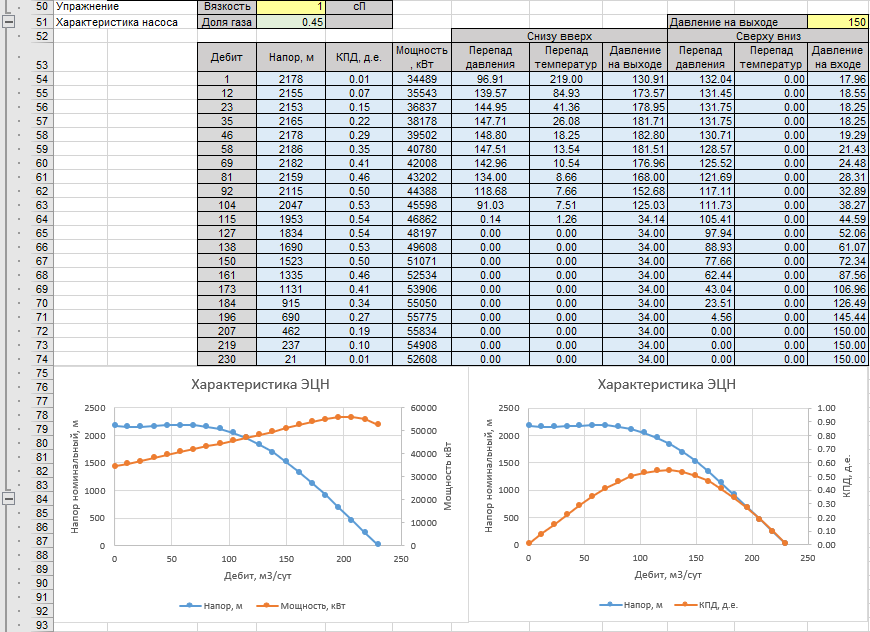
\includegraphics[width=1\linewidth]{Ex70_3}}
	\caption{Напорные характеристики ЭЦН с поправкой на вязкость}
	\label{ris:Ex70_3}
\end{figure}

Расчет перепада давления, развиваемого насосом, может происходить методом "сверху-вниз" \  и "снизу-вверх" \ , при этом расчет перепада температур только методом "снизу-вверх". Функция расчета перепада давления и температуры возвращает массив значений, т.е. одновременно перепад давления и температуры. Кроме того, входным параметром для данной функции является направление расчета. Для вычисления выделите диапазон G54:H54, наберите формулу

{ \small  \texttt{=ESP\_dP\_atm(C54; fw\_; Pintake\_; NumStage\_; Freq\_; PumpID\_; PVTstr; Tintake\_; 0)}}

и после нажмите сочетание клавиш  Ctrl+Shift+Enter. Далее протяните результат до полного заполнения двух столбцов.

Зная давление на приеме и перепад давления в ЭЦН, давление на выходе ЭЦН можно легко посчитать по формуле

{ \small  \texttt{=G54+Pintake\_}}

Предварительно задав давление на выходе ЭЦН в ячейке L51 возможно посчитать перепад давления методом "сверху-вниз"\ аналогичным образом по формуле

{ \small  \texttt{=ESP\_dP\_atm(C54; fw\_; Pdis\_; NumStage\_; Freq\_; PumpID\_; PVTstr; Tintake\_; Tintake\_; 0)}}

И давление на входе, зная давление на выходе и перепад давления

{ \small  \texttt{=Pdis-J54}}

\begin{figure}[h!]
	\center{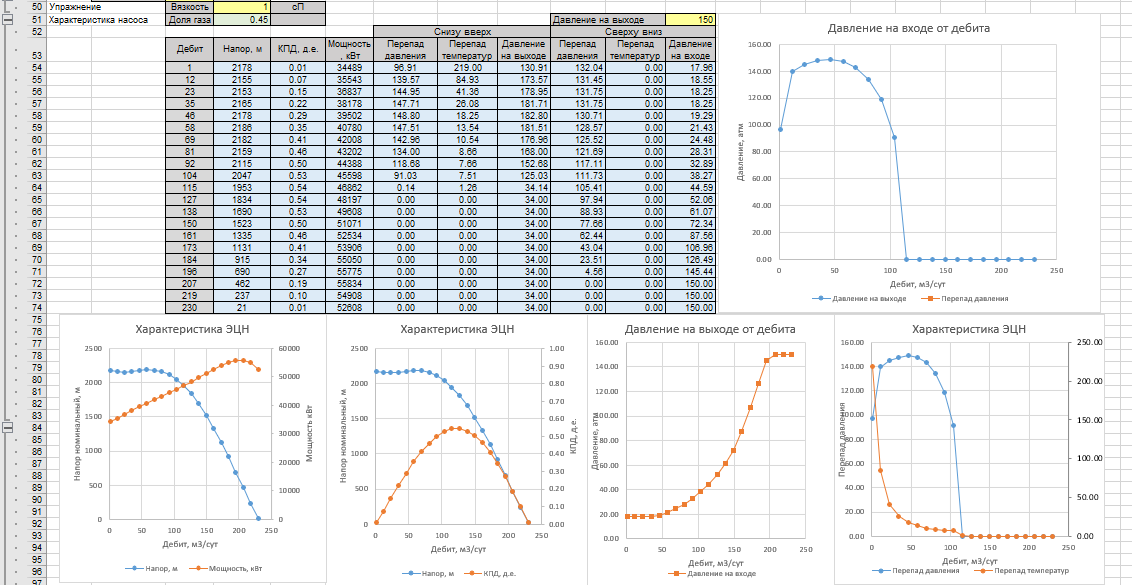
\includegraphics[width=1\linewidth]{Ex70_4}}
	\caption{Расчет перепада давления и температур в ЭЦН в зависимости от дебита}
	\label{ris:Ex70_4}
\end{figure}

Вопросы для упражнения:

\begin{enumerate}
	\item Какие параметры влияют на перепад давления в насосе?
	\item Насколько сильно влияет вязкость на напорные характерситики ЭЦН?
	\item Как влияет на работу ЭЦН изменение частоты?
\end{enumerate}






 % Глава описание упражнений
%	\include{text/conclusion}      % Заключение
%	\include{text/acronyms}        % Список сокращений и условных обозначений
	\chapter*{Словарь терминов}             % Заголовок
\addcontentsline{toc}{chapter}{Словарь терминов}  % Добавляем его в оглавление

Словарь описывает термины и сокращения широко используемые в описании и в системе \unf.


\textbf{VBA} "--- Visual Basic for Application язык программрования встроенный в Excel и использованный для написания макросов \unf.

\textbf{VBE} "--- Среда разработки для языка VBA. Встроена в Excel.

\textbf{BHP, Pwf} "--- Bottom hole pressure. Well flowing pressure. Забойное давление

\textbf{BHT, TBH} "--- Bottom hole temperature. Забойная температура

\textbf{WHP, PWH} "--- Well head pressure. Устьевое давление. Как правило, соответствует буферному давлению.

\textbf{WHT, TWH} "--- Well head temperature. Устьевая температура. Температура флюида на устье скважины. Температура в точке замера буферного давления.

\textbf{IPR} "--- Inflow performance relationship. Индикаторная кривая. Зависимость забойного давления от дебита для пласта. Широко используется в узловом анализе.

\textbf{VLP, VFP} "--- Vertical lift performance, vertical flow performance, outflow curve. Кривая лифта, кривая оттока. Зависимость забойного давления от дебита для скважины. Широко используется в узловом анализе.

\textbf{ESP} "--- Electrical submersible pump. Электрический центробежный насос.

\textbf{GL} "--- Gas Lift. Газлифтный способ эксплуатации добывающих скважин. 

\textbf{РНХ ЭЦН} "--- Расходно напорная характеристика электрического центробежного насоса. Ключевая характеристика ЭЦН. Дается производителем в каталоге ЭЦН для новых насосов или определяется на стенде для ремонтных ЭЦН. 

\textbf{PVT} "--- Pressure Volume Temperature. Общепринятое обозначение для физико-химических свойств пластовых флюидов - нефти, газа и воды.

\textbf{MF} "--- MultiPhase. Много Фазный поток. Префикс для функций имеющих дело с расчетом многофазного потока в трубах и скважине.

\textbf{НКТ} "--- Насосно компрессорная труба. Часть конструкции скважины. по колонне НКТ добывается скважинная продукция или закачивается вода. Может быть заменена в процессе эксплуатации при ремонте скважины. 

\textbf{ЭК} "--- Эксплуатационная колонна. Часть конструкции скважины.  Не может быть заменена в процессе эксплуатации при ремонте скважины. 

\textbf{ГЖС} "--- Газо жидкостная смесь. Часто используется для обозначения совместно двигающихся флюидов в многофазном потоке - нефти, газа, воды.

\textbf{Барботаж, ZNLF} "--- Движение газа через неподвижный столб жидкости. ZNLF - zero net liquid flow. Встречается в скважинах с насосами - в межтрубном пространстве газ движется через неподвижный столб жидкости. Влияет на динамический уровень в скважине.

\textbf{ЭЦН} "--- Электрический центробежный насос.

\textbf{УЭЦН} "--- Установка электрического центробежного насоса. Включает весь комплекс погружного и поверхностного оборудования необходимого для работы насоса - насос (ЭЦН), погружной электрический двигатель (ПЭД), гидрозащита (ГЗ), входной модуль (ВМ) и газосепаратор (ГС), электрический кабель, станция управления (СУ) и другие элементы

\textbf{ЧРП} "--- Частотно регулируемый привод. Элемент УЭЦН обеспечивающий возможность вращения вала УЭЦН с различными частотами.      % Словарь терминов
%	\include{text/references}      % Список литературы
	
	
	%%% Настройки для приложений
%	\appendix
	% Оформление заголовков приложений ближе к ГОСТ:
%	\setlength{\midchapskip}{20pt}
%	\renewcommand*{\afterchapternum}{\par\nobreak\vskip \midchapskip}
%	\renewcommand\thechapter{\Asbuk{chapter}} % Чтобы приложения русскими буквами нумеровались
	
	 % Автоматически сгенерированные листинги программ
%	\include{text/auto_start}
%	\include{text/auto}     

\end{document}
